% Define document class
\documentclass[%
 reprint,
%superscriptaddress,
%groupedaddress,
%unsortedaddress,
%runinaddress,
%frontmatterverbose, 
%preprint,
%preprintnumbers,
 nofootinbib,
%nobibnotes,
%bibnotes,
 amsmath,amssymb,
 aps,
 prd,
%prb,
%rmp,
%prstab,
%prstper,
%floatfix,
]{revtex4-2}
\usepackage[hidelinks]{hyperref}
\usepackage{graphicx}
\usepackage{tabularx}
% \usepackage{subcaption}
% Begin!
\begin{document}

\preprint{APS/123-QED}

\title{BHPWAVE: An adiabatic gravitational waveform model for compact objects undergoing quasi-circular inspirals into rotating massive black holes}% Force line breaks with \\
%\thetaanks{A footnote to the article title}%

\author{Zachary Nasipak}
\affiliation{NASA Goddard Space Flight Center, 8800 Greenbelt Road, Greenbelt, Maryland, 20771, USA}
\email{zachary.nasipak@nasa.gov}

\date{\today}% It is always \today, today,
             %  but any date may be explicitly specified

\begin{abstract}
We present \texttt{bhpwave}: a new Python-based, open-source tool for generating the gravitational waveforms of stellar-mass compact objects undergoing quasi-circular inspirals into rotating massive black holes. These binaries, known as extreme-mass-ratio inspirals (EMRIs), are exciting millihertz gravitational wave sources for future space-based detectors. Relativistic models of EMRI gravitational wave signals are necessary to unlock the full scientific potential of these astrophysical sources, yet few open-source EMRI waveform models exist. To fill this void we built \texttt{bhpwave}, which uses the adiabatic approximation from black hole perturbation theory to rapidly construct gravitational waveforms based on the leading-order inspiral dynamics of the binary. Crucially \texttt{bhpwave} is the first open-source adiabatic model to produce waveforms for binaries with \emph{rotating} massive black holes, opening a new dimension of parameter space for astrophysical investigation.
\end{abstract}

%\keywords{Suggested keywords}%Use showkeys class option if keyword
                              %display desired
\maketitle

% Main body with filler text
\section{Introduction}
\label{sec:intro}

Extreme-mass-ratio inspirals (EMRIs) are binaries composed of a compact object with mass $\mu \sim 10 M_\odot$ inspiraling into a massive black hole with mass $M \sim 10^6 M_\odot$. They emit gravitational waves in the millihertz (mHz) band for months to years, making them promising sources for future space-based detectors, such as the Laser Interferometer Space Antenna (LISA) \cite{NASA11, ESA12}. The prolonged evolution and rich harmonic structure of an EMRI waveform communicates a wealth of information about the binary. Thus, we expect LISA to measure the masses, spins, and orbital characteristics of observed EMRIs with unprecedented accuracy \cite{BabaETC17}. These measurements will provide novel observations of massive black holes and their surrounding environments, while also facilitating high-precision tests of general relativity \cite{BerrETC19}. Extracting this information from an observed signal, however, will likely require subradian-accurate models of EMRI gravitational wave emission. 

Due to their small mass ratios $\epsilon = \mu/M \ll 1$, EMRIs are naturally modeled by black hole perturbation theory and the self-force formalism \cite{PounWard20}. Within this framework, the small body is treated as a perturbation to a background Kerr spacetime. The inspiral of the small body is then driven by a \emph{gravitational self-force} (GSF), which arises from the small body interacting with its own perturbation of the spacetime metric. The metric perturbations and the GSF are constructed perturbatively, order by order in $\epsilon$, to derive the dynamics and resulting gravitational waves radiated by the binary. 

We can understand the relative impact of these self-forces on EMRI gravitational waveforms by expanding the phasing of the EMRI gravitational waveform $\Phi_\mathrm{GW}$ in powers of $\epsilon$ via a two-timescale analysis \cite{HindFlan08},
\begin{align} \label{eqn:twotimescale}
\Phi_\mathrm{GW} = \frac{1}{\epsilon} \left[ \Phi_\mathrm{0PA} + \epsilon^{1/2} \Phi_\mathrm{res} + \epsilon \Phi_\mathrm{1PA} + O(\epsilon^2)\right].
\end{align}
The leading-order \emph{adiabatic} term\footnote{This term is also referred to as the post-0 adiabatic or 0PA term to remain consistent with the naming conventions of the sub-leading terms (e.g., $\Phi_\mathrm{1PA}$).} $\Phi_\mathrm{0PA}$ only depends on the time-averaged \emph{dissipative} first-order GSF, which drives the dissipation of energy and angular momentum from the system. The sub-leading post-1 adiabatic (1PA) piece $\Phi_\mathrm{1PA}$ depends on the remaining contributions from the first-order GSF and the time-averaged components of the second-order GSF. The half-order correction $\Phi_\mathrm{res}$ arises due to the presence of self-forced $r\theta$-resonances experienced by EMRIs undergoing eccentric and inclined inspirals \cite{FlanHind12}. EMRI gravitational models must, therefore, include the $\Phi_\mathrm{0PA}$, $\Phi_\mathrm{res}$, and $\Phi_\mathrm{1PA}$ effects in order to maintain sub-radian phase accuracy and enable the full scientific potential of future mHz gravitational wave observatories. 

Nonetheless purely adiabatic models---which only include $\Phi_\mathrm{0PA}$ in the gravitational wave phasing---may be suitable for detecting (but not characterizing) EMRI signals and are invaluable tools for developing data analysis pipelines for EMRI search and parametrization. They capture almost all of the phasing information and relativistic behavior of EMRI signals, making them powerful probes of astrophysical parameter space. The theoretical foundation and numerical calculation of adiabatic waveforms is also well understood, and has been performed for eccentric, precessing EMRIs \cite{HughETC21}.

In practice, however, it is challenging to optimize adiabatic EMRI waveform calculations in order to make them efficient and accessible, so that they can be incorporated in large scale samplings of parameter space. Currently, only one open-source tool exists for producing adiabatic EMRI waveforms: the Fast EMRI Waveforms (FEW) Python package \cite{ChuaGallVall19, ChuaETC20, KatzETC20, KatzETC21}. While this tool is the gold standard for EMRI waveform models, particularly due to its ability to leverage GPUs, it is currently restricted to eccentric binaries with non-rotating black holes. Since we expect almost all astrophysical EMRIs to possess a rotating massive black hole, this model misses a crucial area of parameter space.

Therefore we introduce \texttt{bhpwave} [RTD link?] an open-source Python-based waveform generator that models the adiabatic dynamics and gravitational wave signals produced by a small body undergoing a quasi-circular\footnote{By ``quasi-circular," we mean that, at any moment of time, the inspiral motion is tangent to a circular geodesic as described in Sec.~\ref{sec:adiabatic}. This is a consequence of the fact that in the adiabatic limit, circular orbits remain circular, i.e., $e(t) = O(\epsilon)$ \cite{KennOri96, Kenn98}.} (non-eccentric) inspiral into a \emph{rotating} massive black hole. This code can model any binary with an initial orbital separation of $r_0 \leq 50 M$ and a massive black hole spin in the range $|a| \leq 0.995 M$. (See Sec.~\ref{sec:adiabatic} for exact definitions of $a$ and $r_0$.) Furthermore, the model supports any mass-ratio, though adiabatic waveform models are most relevant for $\epsilon \lesssim 10^{-4}$. By leveraging parallel computations across CPUs, \texttt{bhpwave} can evaluate years-long waveforms in milliseconds. Even on a standard laptop, waveform evaluations still complete within a few hundred milliseconds to a couple seconds.

A notable limitation of \texttt{bhpwave} is that it currently neglects the effects of eccentricity and precession.\footnote{In a frame where the massive black hole's angular momentum is held fixed, precession is instead described in terms of the inclination of the small body relative to the equatorial plane of the more massive black hole.} Nonetheless, while most observed EMRIs are expected to be highly eccentric \cite{GairETC04},  there are possible formation channels driven by accretion flow that circularize EMRI dynamics and align the orbital angular momentum with the massive black hole's spin \cite{PanLyuYang21}. Thus, \texttt{bhpwave} is applicable to these so-called ``wet-formation" EMRIs. 

Additionally, \texttt{bhpwave} does not provide the first adiabatic calculation of quasi-circular inspirals. These systems have long been studied in the literature \cite{Detw78, KennOri96, FinnThor00, Hugh00b, GralHughWarb16}. However, as aforementioned, it is challenging to implement an adiabatic model that is efficient, reliable, and accessible. Even when neglecting eccentricity, the inclusion of massive black hole spin presents a number of challenges that are less pronounced for binaries with non-spinning bodies, such as the larger range of radial separations accessible to spinning binaries, the faster frequency evolution for more deeply bound orbits, and the higher mode content needed for modeling rapidly-rotating systems. By building upon the theoretical foundations described in the literature, our aim for \texttt{bhpwave} is to provide an efficient and accessible model that fills in this area of parameter space and provides an important stepping stone for developing more advanced models that incorporate all possible orbital effects.

To encourage the continued development of open-source adiabatic EMRI models, this paper outlines the theoretical and numerical foundations underpinning \texttt{bhpwave}. In Sec.~\ref{sec:adiabatic} we summarize the quasi-circular limit of the adiabatic approximation within the context of black hole perturbation theory to establish methods and notation. 
%In Sec.~\ref{sec:bhpwave} we outline how \texttt{bhpwave} implements the quasi-circular adiabatic model, primarily through its three modules: \texttt{bhpwave.trajectory}, \texttt{bhpwave.harmonics}, and \texttt{bhpwave.waveform}. 
In Sec.~\ref{sec:numerical} we describe both the numerical routines used to generate the adiabatic data for \texttt{bhpwave} and the algorithms employed by \texttt{bhpwave} to generate quasi-circular inspirals, waveform harmonics, and gravitational signals. Additionally, we provide validation tests and model comparisons to verify the accuracy of \texttt{bhpwave}. To demonstrate the utility of \texttt{bhpwave}, in Sec.~\ref{sec:errors}, we use a toy problem test the impact of modeling errors on parameter biases for EMRI data analysis. Finally, we discuss further applications and possible extensions of \texttt{bhpwave} in Sec.~\ref{sec:conclusion}. For this paper we use the metric signature $(-+++)$, the sign conventions, where applicable, of \cite{MisnThorWhee73}, and units such that $G=c=1$.


\section{Adiabatic approximation}
\label{sec:adiabatic}

We provide a brief summary of the leading-order adiabatic approximation of a small body's quasi-circular inspiral into a rotating massive black hole. (For extensive discussions of the point-particle and adiabatic approximations see \cite{Hugh00b, Mino03, DrasHugh06, HughETC21} and references therein.) At zeroth-order the small body follows a circular, equatorial geodesic in Kerr spacetime (see \ref{sec:geo}). Due to its mass and motion, the small body excites gravitational radiation. At leading-order this radiation is captured by non-zero perturbations to the Weyl scalar $\psi_4$, which we construct via the Teukolsky equation (see \ref{sec:fluxes}). The resulting flux of energy dissipated via gravitational wave emission---which we compute from $\psi_4$---then drives the decay of the small body's orbital energy and thus the adiabatic inspiral (see \ref{sec:inspiral}). From this inspiral, we then construct the adiabatic gravitational waveform (see \ref{sec:waveform}).

\subsection{Circular, equatorial geodesics}
\label{sec:geo}

Consider a small body with mass $\mu$ orbiting in a Kerr spacetime with metric $g_{\mu\nu}$, which, in Boyer-Lindquist coordinates $(t,r,\theta,\phi)$, is defined by the line element
\begin{multline}
    ds^2 = -\left(1 - \frac{2Mr}{\Sigma} \right) dt^2 - \frac{4Ma r \sin^2\theta}{\Sigma} dtd\phi + \frac{\Sigma}{\Delta} dr^2 
    \\
    + \Sigma d\theta^2 + {\sin^2\theta}\left(r^2+a^2 + \frac{2Ma^2r\sin^2\theta}{\Sigma} \right) d\phi^2,
\end{multline}
where $a$ is the Kerr spin parameter, $M$ is the Kerr mass parameter, $\Delta = r^2 - 2Mr + a^2$, and $\Sigma = r^2+a^2\cos^2\theta$.

The mass $\mu$ follows a geodesic $z_p^\mu \doteq (t_p, r_p, \theta_p, \phi_p)$ that maintains a constant Boyer-Lindquist radius $r_p = r_0$ and is restricted to the equatorial plane $\theta_p = \pi/2$ (with respect to the angular momentum of the Kerr black hole). Due to the Killing symmetries of Kerr spacetime, this motion possesses three constants of motion: the orbital energy $u_t = - \mathcal{E}$, the $z$-component of the orbital angular momentum $u_\phi = \mathcal{L}_z$, and the Carter constant $\mathcal{Q} = Q_{\mu\nu} u^\mu u^\nu$ [citation], which are related to $a$ and $r_0$ by
\begin{subequations} \label{eqn:En}
\begin{align}
    \mathcal{E} &= \frac{1 - 2 v^2 \pm \hat{a} v^3}{\sqrt{1-3v^2\pm 2\hat{a}v^3}},
    \\
    \mathcal{L}_z &= \pm M  \frac{1 \mp 2 \hat{a} v^3 + \hat{a}^2 v^4}{v\sqrt{1-3v^2\pm 2\hat{a}v^3}},
    \\
    \mathcal{Q} &= 0,
\end{align}
\end{subequations}
where $\hat{a} \equiv a/M$, $v^2 = M/r_0$, and $+$ ($-$) refers to prograde (retrograde) orbits.

For circular orbits, the four-velocity $u^\alpha = dz_p^\alpha/d\tau \doteq (\omega_t, 0, 0, \omega_\phi)$ is constant along the geodesic, where $\tau$ is the proper time of the small body. The rates at which (Boyer-Lindquist) time and the azimuthal angle accumulate with $\tau$ are given by
\begin{subequations}
\begin{align}
    \omega_t &= \frac{g_{\phi\phi} \mathcal{E} + g_{t\phi}\mathcal{L}_z}{g_{t\phi}^2-g_{\phi\phi}g_{tt}} = \frac{1 \pm \hat{a} v^3}{\sqrt{1 - 3 v^2 \pm 2 \hat{a} v^3}},
    \\
    \omega_\phi &= -\frac{g_{t\phi} \mathcal{E} + g_{tt}\mathcal{L}_z}{g_{t\phi}^2-g_{\phi\phi}g_{tt}} = \pm \frac{v^3}{M\sqrt{1 - 3 v^2 \pm 2 \hat{a} v^3}},
\end{align}
\end{subequations}
respectively. Straightforward integration then yields
\begin{align*}
    t_p(\tau) &= \omega_t \tau,
    &
    r_p(\tau) &= r_0,
    &
    \theta_p(\tau) &= \frac{\pi}{2},
    &
    \phi_p(\tau) &= \omega_\phi\tau.
\end{align*}
Combining these results, we can re-express the evolution of the orbital phase in terms of coordinate time, $\phi_p(t) = \Omega_p t$, where the geodesic orbital frequency
\begin{equation} \label{eqn:OmegaOfR}
    \Omega_p = \frac{\omega_\phi}{\omega_t}
    = \pm \frac{v^3}{M(1 \pm \hat{a} v^3)}.
\end{equation}
Finally, the innermost stable circular orbit (ISCO) is defined in terms of the minimum radius
\begin{align}
    r_\mathrm{ISCO} &= 3 + z_2 \mp
    \sqrt{(3 - z_1)(3 + z_1 + 2z_2)},
    \\ \notag
    z_1 & = 1 + (1 - \hat{a}^2)^{1/3}
    \left((1-\hat{a})^{1/3} + (1 + \hat{a})^{1/3} \right),
    \\ \notag
    z_2 &= \sqrt{3 \hat{a}^2 + z_1^2},
\end{align}
and maximum frequency $M\Omega_\mathrm{ISCO} = r_\mathrm{ISCO}^{3/2}(M^{3/2} + \hat{a} r_\mathrm{ISCO}^{3/2})^{-1}$.

\subsection{Gravitational wave fluxes}
\label{sec:fluxes}

Next we consider how the small body's motion excites perturbations to the background spacetime. Using the Teukolsky formalism \cite{Teuk73}, we describe these perturbations in terms of the Weyl scalar $\psi_4$, which vanishes in an unperturbed Kerr spacetime and captures two of the ten gravitational degrees of freedom of the metric perturbation. Near infinity, these two degrees of freedom can be related to $h_+$ and $h_\times$ \cite{DrasHugh06}, the two polarizations of the gravitational strain, via
\begin{align} \label{eqn:psi4ToH}
    \psi_4 (r\rightarrow \infty) \simeq \frac{1}{2}(\ddot{h}_+ - i \ddot{h}_\times).
\end{align}
At adiabatic order, $\psi_4$ satisfies the spin-weight $s=-2$ Teukolsky equation (Eq.~(4.7) in \cite{Teuk73}) with a point-particle source (see Sec.~II of \cite{SasaTago03}). The solution is amenable to separation of variables in the frequency-domain, leading to the mode-sum representation
\begin{align} \label{eqn:psi4Modes}
    \psi_4 = \rho^{4} \sum_{j=2}^\infty \sum_{m=-j}^j R_{-2jm}(r) S_{-2jm}(\theta;\gamma) e^{im\phi} e^{-im\Omega_pt},
\end{align}
where $\rho = -(r-ia\cos\theta)^{-1}$, $S_{-2jm}(\theta;\gamma)$ is the spin-weighted spheroidal harmonic of spin-weight $s=-2$ and spheroidicity $\gamma=a m\Omega_p$ (which satisfies Eq.~(2.7) in \cite{TeukPres74}), and $R_{-2jm}(r)$ is the $s=-2$ radial Teukolsky solution (which satisfies Eq.~(3.12) in \cite{DrasHugh06}).

The spin-weighted spheroidal harmonics can be conveniently represented as a rapidly-converging series of spin-weighted spherical harmonics $Y_{s\ell m}(\theta)e^{im\phi}$ \cite{Hugh00b},
\begin{align}
    S_{sjm}(\theta, \gamma) = \sum_{\ell=\ell_\mathrm{min}}^\infty b_{sjm}^\ell(\gamma) Y_{s\ell m}(\theta),
\end{align}
where $\ell_\mathrm{min}=\mathrm{max}[|m|,|s|]$. This decomposition is particularly useful because it allows us to reproject $\psi_4$ onto an angular basis that is independent of frequency,
\begin{align} \label{eqn:psi4LModes}
    \psi_4 = \rho^{4} \sum_{\ell=2}^\infty \sum_{m=-\ell}^\ell X_{-2\ell m}(r) Y_{-2\ell m}(\theta)e^{im(\phi - \Omega_pt)},
\end{align}
where
\begin{align} \label{eqn:XfromR}
    X_{-2\ell m}(r) = \sum_{j=\ell_\mathrm{min}}^\infty b_{-2jm}^\ell(\gamma)R_{-2jm}(r).
\end{align}
Furthermore, the spin-weighted spherical harmonics form a complete and orthonormal set of basis functions on the unit sphere (for the same value of spin-weight),
\begin{align}
    \int Y_{s\ell m} {Y}_{s\ell'm'} e^{i(m-m')\phi} d\Omega = \delta_{l l'} \delta_{m m'}.
\end{align}

%In general, the spin-weighted spheroidal harmonics satisfy,
% \begin{multline}
%     \Bigg[\frac{1}{\sin\theta}\frac{d}{d\theta}\left(\sin\theta \frac{d}{d\theta} \right)
%     - \bigg(\gamma^2\sin^2\theta -2m\gamma -s
%     \\
%     +\frac{(m+s\cos\theta)^2}{\sin^2\theta}
%     +2\gamma s\cos\theta -\lambda_{sjm\gamma} \bigg) \Bigg]S_{sjm\gamma} = 0,
% \end{multline}
% with eigenvalue $\lambda_{sjm\gamma}$. Therefore, we restrict ourselves to the case $S_{-2jm} = S_{-2jm(\gamma=am\Omega_p)}$. 

% For general spin-weight $s$ and frequency $\omega$, the radial Teukolsky solution satisfies
% \begin{align}
%     \left[\Delta^{-s} \frac{d}{dr} \left(\Delta^{s+1} \frac{d}{dr}  \right)
% 	+ V_{sjm\omega}(r)\right]R_{sjm\omega}(r) = T_{sjm\omega}(r)
% \end{align}
% where
% \begin{align}
%     V_{sjm\omega} &= \frac{K^2+4i(r-M)K}{\Delta}-8i\omega r - \lambda_{sjm(a\omega)},
% \end{align} 
% $K = (r^2+a^2)\omega - ma$, and the source term $T_{sjm\omega}$ is given in \cite{Teuk73}. 

For our point-particle source on a circular geodesic, the radial mode function $R_{-2jm}(r)$ have the asymptotic forms
\begin{subequations} \label{eqn:asympR}
\begin{align}
    R_{-2jm}(r\rightarrow r_+) &\simeq Z^\mathcal{H}_{-2jm} \Delta^{2} e^{-im k_p r_*},
    \\ 
    R_{-2jm}(r\rightarrow \infty) &\simeq Z^\mathcal{I}_{-2jm} r^{3} e^{+im\Omega_p r_*},
\end{align}
\end{subequations}
where $k_p = \Omega_p - \Omega_+$, the horizon frequency $\Omega_+ = a/(2Mr_+)$, and the tortoise coordinate $r_*$ is given by the differential relation $dr_*/dr = (r^2+a^2)/\Delta$.
The amplitudes $Z^\mathcal{H/I}_{-2jm}$ are often referred to as \emph{Teukolsky amplitudes} and are constructed via the standard Green's function method, also known as the method of variation of parameters (see Sec.~III\,A in \cite{HughETC21} or \cite{DrasHugh06} for further details). From \eqref{eqn:XfromR}, we see that $X_{-2\ell m}$ then possesses the same asymptotic behavior as $R_{-2\ell m}$ in \eqref{eqn:asympR} but with modified amplitudes
\begin{align}
    Z^\mathcal{H/I}_{-2jm} \rightarrow X^\mathcal{H/I}_{-2\ell m} = \sum_{j=\ell_\mathrm{min}}^\infty b^\ell_{-2jm}(\gamma) Z^\mathcal{H/I}_{-2jm}.
\end{align}
As a final note, because $Z^\mathrm{H/I}_{-2jm}$ and  $X^\mathrm{H/I}_{-2\ell m}$ depend on the source motion, we can parametrize both amplitudes in terms of the orbital constants, e.g., $X^\mathcal{H/I}_{-2\ell m}= {X}^\mathcal{H/I}_{-2\ell m}(\Omega_p; a)$.

Upon obtaining $\psi_4$, we can then calculate the flux of energy that $\psi_4$ radiates away to infinity $\dot{E}^\mathcal{I}$ and down the black hole horizon $\dot{E}^\mathcal{H}$ \cite{TeukPres74}, 
\begin{subequations} \label{eqn:fluxes}
\begin{align}
    \dot{E}^\mathcal{I} &= \frac{1}{4\pi} \sum_{jm} \alpha_{jm}^\infty {|Z^\mathcal{I}_{-2jm}|^2},
    \\
    \dot{E}^\mathcal{H} &= \frac{1}{4\pi} \sum_{jm} \alpha_{jm}^\mathcal{H} {|Z^\mathcal{H}_{-2jm}|^2},
\end{align}
\end{subequations}
where 
\begin{align*}
    \alpha_{jm}^\mathcal{I} &= \frac{1}{m^2\Omega_p^2},
    \\
    \alpha_{jm}^\mathcal{H} &= \frac{256m^2 k_p\Omega_p(2Mr_+)^5(m^2k_p^2+4\epsilon^2)(m^2k_p^2+16\epsilon^2)}{|C_{2jm}|^2},
\end{align*}
$\epsilon = (r_+ - M)/(2Mr_+)$, and the Teukolsky-Starobinsky constant is given by
\begin{align} 
    |C_{2jm}|^2 &=\Lambda_{2j m }^2(\Lambda_{2j m }-2)^2
    \\ \notag
    & \quad + 8 a m^2 \Omega_p(1 - a \Omega_p)(\Lambda_{2j m }-2)(5\Lambda_{2j m }-4)
    \\ \notag
    & \quad \quad
    +48 (a m \Omega_p)^2[4(\Lambda_{2j m }-1)+3m(1- a \Omega_p)].
\end{align}
Note that the Chandrasekhar eigenvalue $\Lambda_{sjm} = \lambda_{sjm} + s(s+1)$ is invariant under the interchange $s\rightarrow -s$ \cite{Chan83}.
The angular momentum fluxes are then related to the energy fluxes by $\dot{L}_z^{\mathcal{I}/\mathcal{H}} = \Omega^{-1} \dot{E}^{\mathcal{I}/\mathcal{H}}$, leading to the total gravitational wave fluxes
\begin{align}
    \dot{E}^\mathrm{GW} &= \dot{E}^\mathcal{I} + \dot{E}^\mathcal{H},
    &
    \dot{L}_z^\mathrm{GW} &= \dot{L}_z^\mathcal{I} + \dot{L}_z^\mathcal{H}.
\end{align}

\subsection{Adiabatic quasi-circular inspirals}
\label{sec:inspiral}

Due to gravitational {radiation-reaction}, the small body does not remain on a circular geodesic. The binary {radiates} gravitational waves and the small body {reacts} to the radiative losses of energy and angular momentum by undergoing a quasi-circular inspiral into the rotating massive black hole. We can parametrize this motion in terms of the time-evolving orbital energy ${E}(t)$ and orbital phase $\Phi(t)$ of the inspiraling body, which at leading order is given by the equations of motion \cite{PounWard20,HughETC21},
\begin{align} \label{eqn:eom}
    \frac{d {E}}{dt} &= -\epsilon \mathcal{F}_E + O(\epsilon^2),
    &
    \frac{d\Phi}{dt} &= \Omega + O(\epsilon).
\end{align}
Because $\dot{E} \sim \epsilon$, the orbital energy evolves gradually and the evolution can be understood in terms of the \emph{osculating geodesics} method \cite{GairETC11}. At any time $t_0$, the motion is approximately tangent to a geodesic with energy $E(t_0) \approx \mathcal{E}$ and frequency $\Omega(t_0) \approx \Omega_p$. The small body then evolves from geodesic to geodesic based on its gravitational wave emission until the body approaches the ISCO, at which point the approximation breaks down and we end the evolution.

In effect, at leading order we can express the orbital frequency $\Omega$ in terms of the orbital energy ${E}$ using Eqs.~\eqref{eqn:En} and \eqref{eqn:OmegaOfR}, but with $\mathcal{E}$ and $\Omega_p$ replaced by $E$ and $\Omega$, respectively. Furthermore, the forcing term $\mathcal{F}_E$ is constructed using flux-balance arguments \cite{Mino03, Galt82, QuinWald99}: for a point-particle on a circular geodesic the loss of orbital energy is balanced by the gravitational wave energy flux $\dot{E}^\mathrm{GW}$, leading to the relation $\epsilon \mathcal{F}_E = \dot{E}^\mathrm{GW}$. 

As seen from Eq.~\eqref{eqn:eom}, the time it takes the system to undergo this inspiral scales with the radiation reaction timescale $T_\mathrm{insp} \sim T_\mathrm{rr} = M \epsilon^{-1}$. Similarly, the total accumulated phase scales like $\Delta\Phi_\mathrm{insp} \sim \epsilon^{-1}$, thus giving the leading-order phase contribution to the gravitational wave signal, as described in Eq.~\eqref{eqn:twotimescale}.

\subsection{Time domain adiabatic waveform}
\label{sec:waveform}

After determining the adiabatic inspiral of the smaller body, we generalize \eqref{eqn:psi4LModes}---our geodesic expression for $\psi_4$---by once again leveraging the fact that at any moment of time the motion is approximately tangent to a geodesic. Consequently, the field amplitudes are promoted from constants to quantities that slowly evolve with frequency and time $X^\mathcal{H/I}_{-2\ell m}(\Omega_p; a) \rightarrow X^\mathcal{H/I}_{-2\ell m}(\Omega(t); a)$, while the field's phase rapidly accumulates in proportion to the orbital phase $\Omega_p t \rightarrow \Phi(t)$. As a result, the adiabatic waveform $h = h_+ - i h_\times$ takes the form
\begin{subequations} \label{eqn:adiabaticWaveform}
\begin{align} 
    h(u,r,\theta,\phi) &= \frac{\mu}{r}\sum_{\ell m} h_{\ell m}(u,r,\theta,\phi),
    \\
    h_{\ell m}(u,r,\theta,\phi) & = B_{\ell m}(u) Y_{-2\ell m}(\theta) e^{im[\phi - \Phi(u)]}  
\end{align}
\end{subequations}
where, assuming $r \gg M$, the waveform amplitudes are given by
\begin{align} \label{eqn:amplitude}
    B_{\ell m}(u) = -2\frac{X_{-2\ell m}^\mathcal{I}( \Omega(u);a)}{m^2\Omega^2(u)} = A_{\ell m} e^{i \psi_{\ell m}}.
\end{align}
For later convenience we introduce the magnitude of the waveform amplitudes $A_{\ell m} = |B_{\ell m}|$ and the phase of the complex amplitudes $\psi_{\ell m}$, both of which depend on $\Omega(u)$ and $a$. Furthermore, rather than using the conventions of \cite{KatzETC21,HughETC21}, we follow \cite{PounWard20} and parametrize the adiabatic waveform in terms of the outgoing time-coordinate $u=t-r_*$. As a result, if we hold the orbital constants and frequencies fixed, \eqref{eqn:adiabaticWaveform} reduces to a geodesic ``snapshot'' waveform obtained via \eqref{eqn:psi4ToH} and \eqref{eqn:psi4LModes}. In practice, when implementing \eqref{eqn:adiabaticWaveform} in \texttt{bhpwave}, we replace $u$ with Boyer-Lindquist time $t$ to match the FEW model (which is described by (10) in \cite{KatzETC21}). This is equivalent to parametrizing all of our waveforms with an initial time $t_0 = r_*$.

\subsection{Frequency domain waveforms}

The amplitude and phase decomposition of \eqref{eqn:adiabaticWaveform} makes it particularly straightforward to represent our waveforms in the frequency domain via the stationary phase approximation \cite{HughETC21},
\begin{subequations} \label{eqn:fourierH}
\begin{align}
    \tilde{h}(f) &= \int_{-\infty}^\infty h(t) e^{2\pi i f t} dt,
    \\ 
    &=  \frac{\mu}{r}\sum_{\ell m}\tilde{h}_{\ell m}(f),
    \\ 
    \tilde{h}_{\ell m}(f) & \approx \tilde{B}_{\ell m}(f) Y_{-2\ell m} e^{i[2\pi f t_p(f)+ m(\phi-\Phi[t_p(f)])]},
\end{align}
\end{subequations}
where
\begin{align} \label{eqn:fourierAmplitude}
    \tilde{B}_{\ell m}(f) \approx \sqrt{\frac{2\pi}{i m \dot{\Omega}[t_p(f)]}} {B}_{\ell m}(t_p(f)),
\end{align}
and $t_p(f)$ refers to the times at which the binary emits gravitational waves with frequency $f$. For each $(\ell, m)$-mode, time and frequency are (approximately) related by
\begin{align} \label{eqn:fourierPhase}
    2\pi f \approx m \dot{\Phi}(t) = m \Omega(t),
\end{align}
which we can invert to obtain $t_p(f)$ for individual harmonics. Both \eqref{eqn:fourierAmplitude} and \eqref{eqn:fourierPhase} neglect terms related to $\dot{\psi}_{\ell m}$ and $\ddot{\psi}_{\ell m}$, which introduces an $O(\epsilon)$ error to the phase and an $O(\epsilon^{1/2})$ error to the amplitude. (See Appendix \ref{app:fourierPhase} for further details.) Since the amplitudes scale as $\tilde{B}_{\ell m}(f) \sim 1/\sqrt{\epsilon}$, it is safe to neglect these terms for small mass-ratios.

\section{Solar system barycenter waveforms}

Up to this point, waveforms have been constructed in the source frame, with our Boyer-Lindquist coordinate system centered on the massive black hole. To get the observed waveform in the solar system barycenter (SSB) frame $h_\mathrm{SSB}$, we adopt the same conventions as the \textsc{FEW} model and make use of the transformation provided in \cite{KatzETC21}. In this frame, 
a generic EMRI system is parametrized by 12 intrinsic parameters $(\mu, M, a, \vec{a}_2, p_0, e_0, x_0, \Phi_{r0}, \Phi_{\theta 0}, \Phi_{\phi 0})$---where $\vec{a}_2$ is the spin-vector of the smaller body; $p_0$, $e_0$, and $x_0$ are respectively the initial semi-latus rectum, orbital eccentricity, and projection of the orbital inclination; and $\Phi_{r0}$, $\Phi_{\theta 0}$, $\Phi_{\phi 0}$ are respectively the initial radial, polar, and azimuthal phases---and by 5 extrinsic parameters $(d_L, q_S, \phi_S, q_K, \phi_K)$---where $d_L$ is the luminosity distance to the source EMRI, $q_S$ and $\phi_S$ are the polar and azimuthal sky positions of the source, and $q_K$ and $\phi_K$ are the polar and azimuthal angles defining the orientation of the massive black hole's axis of rotation. In our simplified quasi-circular setup, five of the intrinsic parameters are constrained to the values $\vec{a}_2 = \vec{0}$, $e_0 = 0$, $x_0 = 1$, $\Phi_{r0} = \Phi_{\theta 0} = 0$, while two of the remaining free intrinsic parameters are given by $\Phi_{\phi 0} = \Phi(0)$ and $p_0 = r_0$.

The extrinsic parameters are related to Boyer-Lindquist $(r,\theta, \phi)$ via
\begin{subequations} \label{eqn:SSBtoSource}
    \begin{align}
        r &= d_L,
        \\
        \cos\theta &= - \cos q_S\cos q_K
        \\ \notag
        & \qquad \quad -\sin q_S \sin q_K \cos(\phi_K - \phi_S),
        \\
        \phi &= -\frac{\pi}{2}.
    \end{align}
\end{subequations}
The frame transformation also rotates the polarization basis by the polarization angle $\psi$ \cite{KatzETC21}. As a result, $h_\mathrm{SSB}$ is related to $h$, the strain in the source frame, via
\begin{align} \label{eqn:polarization}
    h_\mathrm{SSB} = e^{2i\psi} h = \frac{D_\psi^2}{|D_\psi|^2} h = \frac{D_\psi}{D^*_\psi} h,
\end{align}
where $D_\psi$ is given by
\begin{multline}
    D_\psi = \cos q_S \sin q_K \cos(\phi_K - \phi_S)
    \\ 
     - \sin q_S\cos q_K +i \sin q_K \sin(\phi_K - \phi_S),
\end{multline}
and $a^*$ denotes the complex conjugate of $a$. Note that there are two cases in which the preferred wave basis in \cite{KatzETC20} is no longer uniquely defined: $(q_K, \phi_K) = (q_S, \phi_S)$ and $(q_K, \phi_K) = (\pi - q_S, \pi + \phi_S)$. In both instances the SSB and source frames are aligned or anti-aligned with one another, leading to $D_\psi = 0$ and invalidating the last equality in \eqref{eqn:polarization}. Therefore, we choose $h_\mathrm{SSB} = h$ if $(q_K, \phi_K) = (q_S, \phi_S)$ or $(q_K, \phi_K) = (\pi - q_S, \pi + \phi_S)$.



\section{Numerical methods}
\label{sec:numerical}

\subsection{Equations of motion and the numerical domain}

To simplify the calculation of our inspirals, we introduce the dimensionless and rescaled orbital quantities
\begin{align}
    \check{t} &= \frac{\mu t}{M^2},
    &
    \check{\Phi} &= \frac{\mu \Phi}{M},
    &
    \hat{\Omega} &= M \Omega,
    &
    \hat{a} &= \frac{a}{M}.
\end{align} 
A hat represents a quantity that is made dimensionless, while a check represents a quantity that is dimensionless and scaled by the mass ratio. We then reparametrize the equations of motion in terms of the (dimensionless) orbital frequency, yielding
\begin{subequations} \label{eqn:eom1}
\begin{align} \label{eqn:dtdOmega}
    \frac{d\hat{\Omega}}{d\check{t}} &= -\left[\partial_{\mathcal{E}}\hat{\Omega}(\hat{\Omega}; \hat{a}) {\mathcal{F}}_E(\hat{\Omega}; \hat{a})\right],
    \\ \label{eqn:dPhidOmega}
    \frac{d\check{\Phi}}{d\check{t}} &= \hat{\Omega},
\end{align} 
\end{subequations}
for time-domain trajectories, and 
\begin{subequations} \label{eqn:eom2}
\begin{align} \label{eqn:dtdOmega}
    \frac{d\check{t}}{d\hat{\Omega}} &= -\left[\partial_{\mathcal{E}}\hat{\Omega}(\hat{\Omega}; \hat{a}) {\mathcal{F}}_E(\hat{\Omega}; \hat{a})\right]^{-1},
    \\ \label{eqn:dPhidOmega}
    \frac{d\check{\Phi}}{d\hat{\Omega}} &= -\hat{\Omega} \left[\partial_{\mathcal{E}}\hat{\Omega}(\hat{\Omega}; \hat{a}) {\mathcal{F}}_E(\hat{\Omega}; \hat{a})\right]^{-1},
\end{align} 
\end{subequations}
for the frequency domain.
The Jacobian $\partial_{\mathcal{E}}\hat{\Omega}$ is analytically obtained from \eqref{eqn:En} and \eqref{eqn:OmegaOfR}, while we construct ${\mathcal{F}}_E$ numerically via \eqref{eqn:fluxes}.

In this form, the equations of motion no longer depend on the masses of the binary, just the dimensionless orbital frequency and dimensionless Kerr spin parameter. By parametrizing in terms of frequency in \eqref{eqn:eom2}, we decouple the evolution in time and phase, leading to solutions $\check{t}(\hat{\Omega}; \hat{a})$ and $\check{\Phi}(\hat{\Omega}; \hat{a})$. In this form, it is straightforward to construct the frequency domain waveforms via Eqs.~\eqref{eqn:fourierH}-\eqref{eqn:fourierPhase}.

% Calculating time-domain waveforms then requires either inverting (i.e., $\check{t}(\hat{\Omega}; \hat{a}) \rightarrow \hat{\Omega}(\check{t}; \hat{a})$) or solving the inverse of \eqref{eqn:dtdOmega} (i.e.,  $d\hat{\Omega}/d\check{t} = \left[d\check{t}/d\hat{\Omega} \right]^{-1}$). In this work, we perform the former to avoid $d\hat{\Omega}/d\check{t}$ diverging at the ISCO.

Therefore, we first interpolate the data $\mathcal{F}_E(\hat{\Omega}; \hat{a})$, and then solve the equations of motion for the rescaled frequency-domain trajectories $\check{t}(\hat{\Omega}; \hat{a})$ and $\check{\Phi}(\hat{\Omega}; \hat{a})$. We set the initial conditions $\check{t}(\hat{\Omega}_\mathrm{ISCO}) = \check{\Phi}(\hat{\Omega}_\mathrm{ISCO}) = 0$. Thus all time and phase values are $\leq 0$. We then solve for the time-domain trajectories $\hat{\Omega}(\check{t}; a)$ and $\check{\Phi}(\check{t}; a)$. Data can be precomputed and stored on a numerical grid spanning the domains of $(\hat{a}, \hat{\Omega})$ or $(\hat{a}, \check{t})$. From these grids, we construct bicubic spline interpolants to represent the trajectories, which can be rapidly evaluated to get any quasi-circular inspiral within our domain. For this work, we set the boundaries of our grid at $\hat{a} \in [-\hat{a}_\mathrm{max}, +\hat{a}_\mathrm{max}]$ and $\hat{\Omega} \in [\hat{\Omega}_\mathrm{min}, \hat{\Omega}_\mathrm{ISCO}]$ with $\hat{a}_\mathrm{max} = 0.9999$ and $\hat{\Omega}_\mathrm{min} = 2\times 10^{-3}$ (which corresponds to $r_0 \approx 60 M$). This domain is plotted in Fig.~\ref{fig:domain}.

Note that, due to the one-to-one mapping between time and frequency, we could calculate the frequency-domain trajectories and then invert them to get the time-domain trajectories. In practice, however, we create four separate spline representations for $\check{t}(\hat{\Omega}; \hat{a})$, $\check{\Phi}(\hat{\Omega}; \hat{a})$, $\hat{\Omega}(\check{t}; a)$, and $\check{\Phi}(\check{t}; a)$. This is much more computationally efficient then inverting one set of solutions through root-finding methods (e.g., $\hat{\Omega}(\check{t}_0) = \mathrm{Root}[\check{t}(\hat{\Omega}) - \check{t}_0]$) and avoids the accumulation of interpolation errors when taking the composition of two splines (e.g., $\check{\Phi}(\check{t}_0) = \check{\Phi}[\hat{\Omega}(\check{t}_0)])$.

\begin{figure}
    \centering
    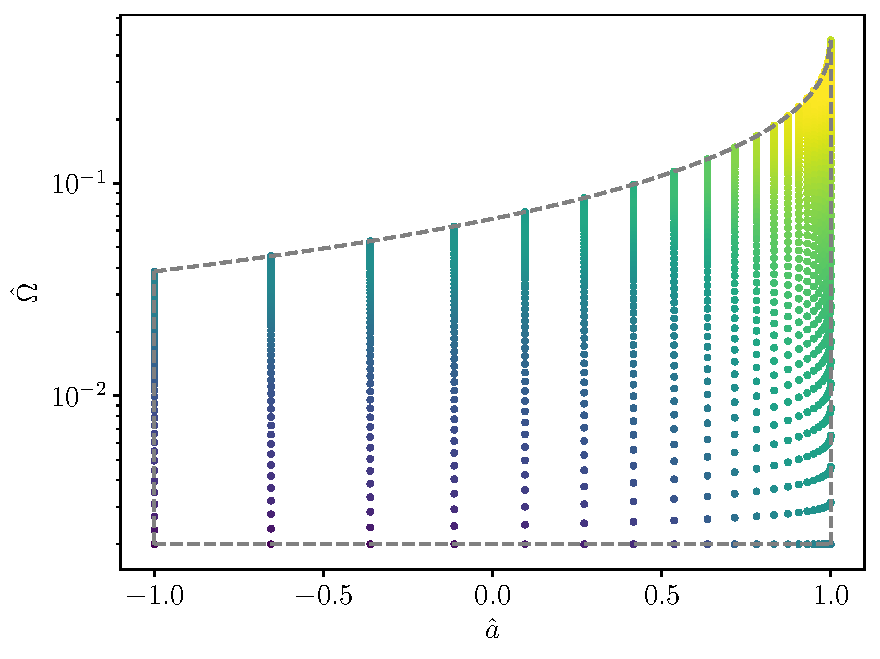
\includegraphics[width=0.95\columnwidth]{figures/domain_sampling.pdf}
    \caption{A $32\times 64$ grid in $(\alpha, \chi)$ mapped to the $(\hat{a}, \hat{\Omega})$ domain. Each dot represents a sampled point in the parameter space. These points are equally-spaced in $\alpha$ and in $\chi$, but cluster around $\hat{\Omega} = \hat{\Omega}_\mathrm{ISCO}$ and $\hat{a} = \hat{a}_\mathrm{max}$. The shading of each point reflects the relative density of points in the $(\hat{a}, \hat{\Omega})$ domain, while the dashed lines represent the domain boundaries.}
    \label{fig:domain}
\end{figure}

\subsection{Interpolated fluxes and trajectories}

There are two main challenges to constructing $\mathcal{F}_E(\hat{\Omega}; \hat{a})$ via numerical interpolation: (1) the lower frequency boundary $\hat{\Omega}=\hat{\Omega}_\mathrm{ISCO}$ has a particularly strong dependence on the black hole spin as highlighted in Figure \ref{fig:domain}; and (2) $\mathcal{F}_E$, $\check{t}$, and $\check{\Phi}$ rapidly accumulate as $\hat{\Omega} \rightarrow \hat{\Omega}_\mathrm{ISCO}$ and $\hat{a} \rightarrow 1$ as shown in Figure \ref{fig:original}. A simple uniform sampling in $\hat{a}$ and $\hat{\Omega}-\hat{\Omega}_\mathrm{ISCO}$ could lead to substantial errors in our interpolating functions due to the large magnitudes of the higher-order derivatives with respect to $\hat{a}$ and $\hat{\Omega}$.

Consequently, we alter our parametrization to mitigate errors in our numerical spline interpolations. We first ameliorate the growth in flux, time, and phase by rescaling $\mathcal{F}_E$, $\check{t}$, and $\check{\Phi}$ by their frequency-dependence at leading post-Newtonian order,
\begin{align}
    \mathcal{F}_E^\mathrm{PN} &= \hat{\Omega}^{10/3},
    \\
    \check{\Phi}^\mathrm{PN} &= \hat{\Omega}_\mathrm{ISCO}^{-5/3} - \hat{\Omega}^{-5/3},
    \\
    \check{t}^\mathrm{PN} &= \hat{\Omega}_\mathrm{ISCO}^{-8/3} - \hat{\Omega}^{-8/3},
\end{align}
resulting in the normalized functions
\begin{align}
    \mathcal{F}_N &= \frac{\mathcal{F}_E}{\mathcal{F}_E^\mathrm{PN}},
    &
    \check{\Phi}_N &= \frac{\check{\Phi}}{ \check{\Phi}^\mathrm{PN} + \delta},
    &
    \check{t}_N &= \frac{\check{t}}{\check{t}^\mathrm{PN} + \delta},
\end{align}
which are plotted in the middle panel of Fig.~\ref{fig:rescaled}. We introduce the $\delta = 10^{-6}$ offset to avoid division by zero as $\hat{\Omega} \rightarrow \hat{\Omega}_\mathrm{ISCO}$. As a result of this shift, the normalized time and phase data still satisfy the initial conditions $\check{t}_N(\hat{\Omega}_\mathrm{ISCO}) = \check{\Phi}_N(\hat{\Omega}_\mathrm{ISCO}) = 0$. Next, motivated by post-Newtonian and near-extremal expansions of the orbital quantities, we introduce $x = \hat{\Omega}^{1/3}$ and $y = (1 - \hat{a})^{1/3}$, from which we define the final sampling parameters,
\begin{align} \label{eqn:params}
    \alpha^2 &= \frac{x_\mathrm{ISCO}-x}{x_\mathrm{ISCO}-x_\mathrm{min}},
    &
    \chi^2 &= \frac{y-y_-}{y_+-y_-},
\end{align}
where $x_\mathrm{min} = \Omega_\mathrm{min}^{1/3}$, $x_\mathrm{ISCO} = \Omega_\mathrm{ISCO}^{1/3}$, and $y_\pm = (1 \pm a_\mathrm{max})^{1/3}$. We square the left-hand side of \eqref{eqn:params} to further smooth out the behavior near the ISCO and maximal spin values. This can be seen in Fig.~\ref{fig:final}, where we plot the variation in $\check{t}$ and $\check{\Phi}$ with respect to $\alpha$ and $\chi$.

\begin{figure*}[!htp]
    \centering
    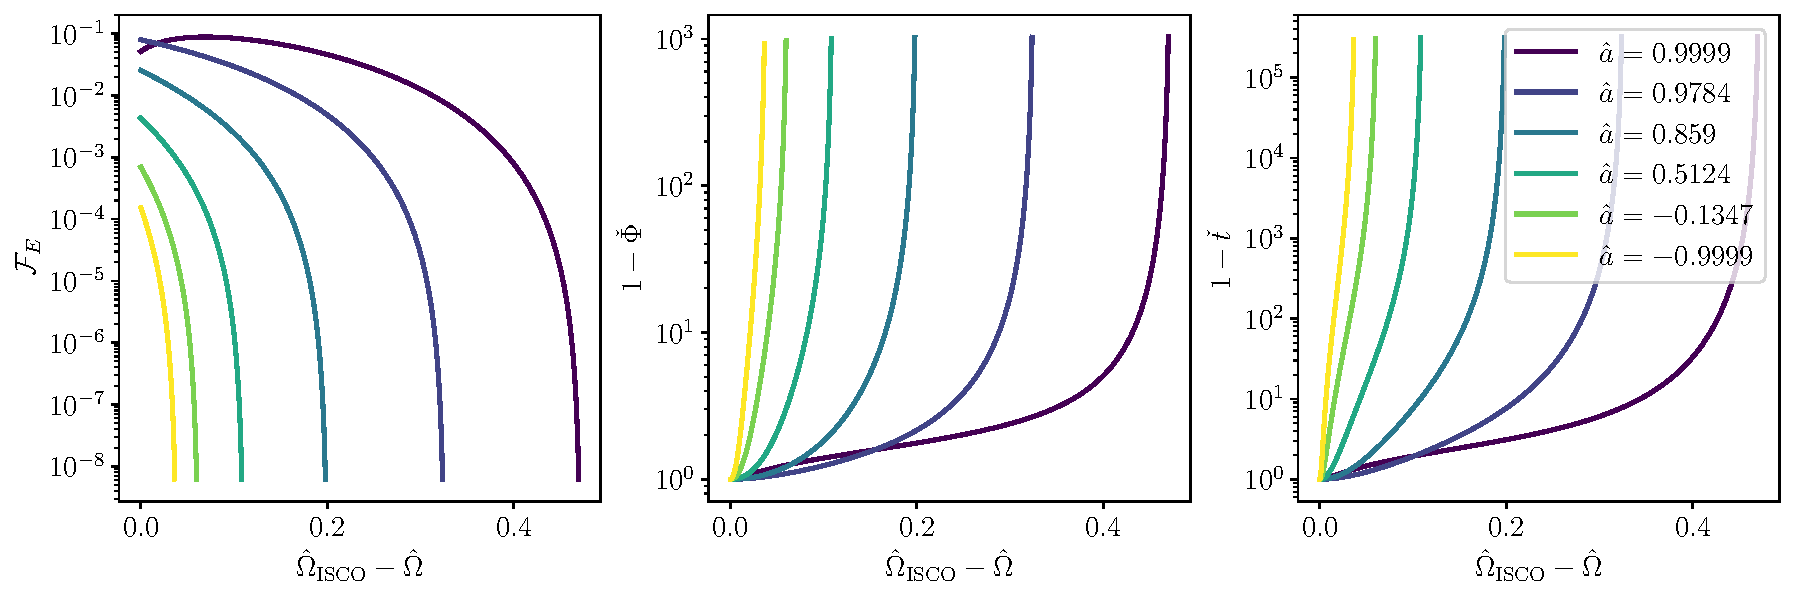
\includegraphics[width=0.95\linewidth]{figures/orginal_parametrization.pdf}
    \caption{Different rescalings and reparametrizations of the flux to improve interpolation accuracy of the numerical data.}
    \label{fig:original}
\end{figure*}

\begin{figure*}[!htp]
    \centering
    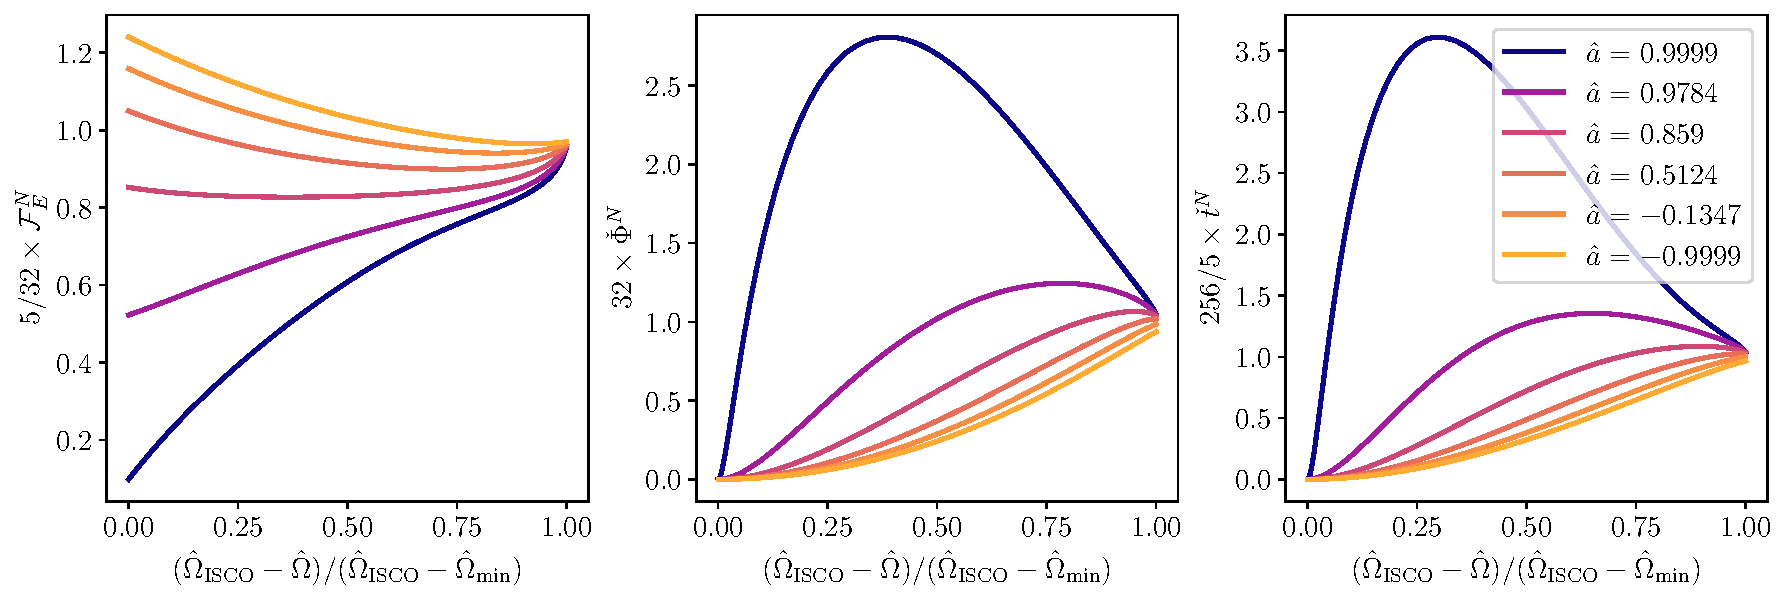
\includegraphics[width=0.98\linewidth]{figures/rescaled_parametrization.pdf}
    \caption{Different rescalings and reparametrizations of the flux to improve interpolation accuracy of the numerical data.}
    \label{fig:rescaled}
\end{figure*}

\begin{figure*}[!htp]
    \centering
    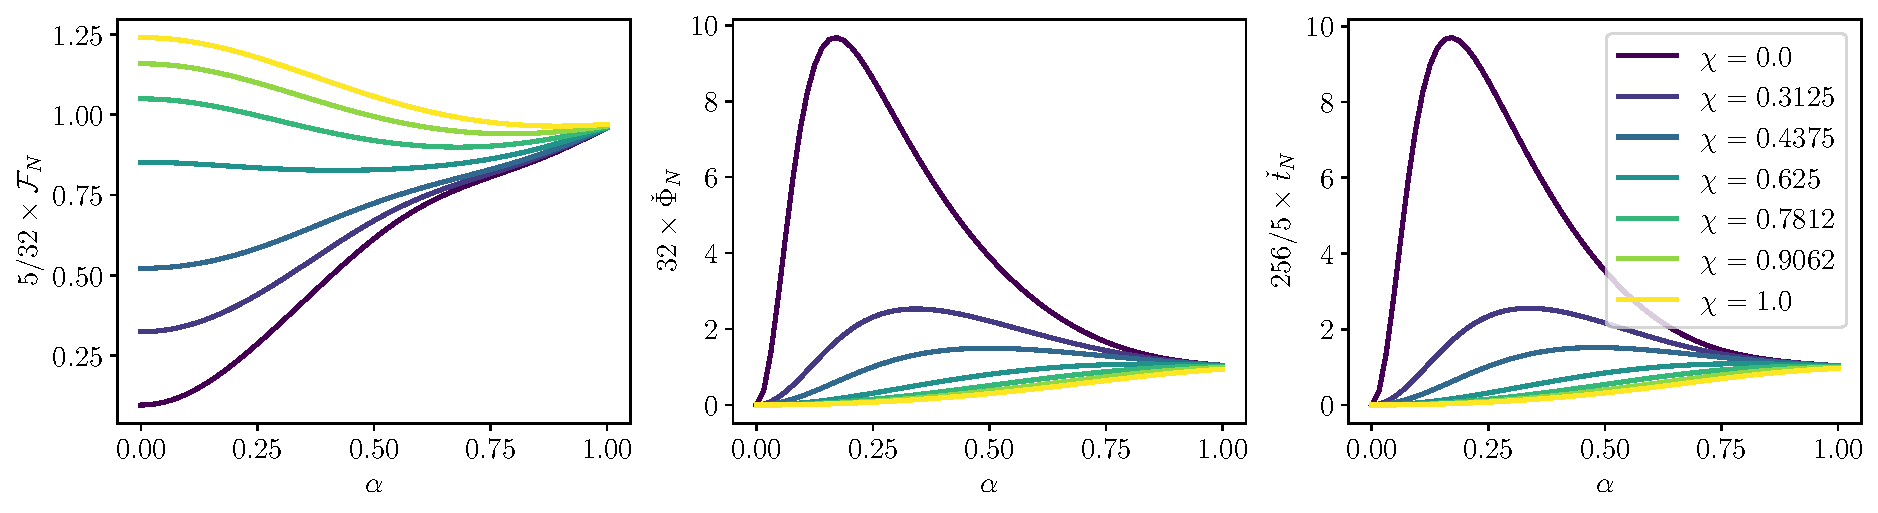
\includegraphics[width=0.98\linewidth]{figures/final_parametrization.pdf}
    \caption{Different rescalings and reparametrizations of the flux to improve interpolation accuracy of the numerical data.}
    \label{fig:final}
\end{figure*}

After choosing this parametrization, we solve for the fluxes $\dot{E}^\mathrm{GW}$ using the Teukolsky solver provided in the \texttt{pybhpt} Python package.\footnote{This code is available at \href{https://github.com/znasipak/pybhpt}{github.com/znasipak/pybhpt}.} Flux data is calculated with a requested precision of $10^{-10}$. We precompute $\dot{E}^\mathrm{GW}$, from which we get $\mathcal{F}_E$, on a fixed grid in the $(\alpha, \chi)$ domain using 129 equally-spaced samples in $\chi$ and 257 equally-spaced samples in $\alpha$. A downsampling of these points is mapped to the $(\hat{a}, \hat{\Omega})$ domain in Fig.~\ref{fig:domain} to illustrate the concentration of sampling points towards the ISCO and near-extremal spins. From this grid, we construct the interpolated function $\mathcal{F}_N^I(\alpha, \chi)$, then solve \eqref{eqn:eom2} for $\check{t}$ and $\check{\Phi}$ on a more densely sampled $513 \times 513$ grid in $(\alpha, \chi)$. We then assemble the interpolated functions $\check{t}^I_{N}(\alpha, \chi)$ and $\check{\Phi}^I_{N}(\alpha, \chi)$. Note that we explicitly differentiate between numerical solutions and their interpolated approximants by labeling interpolated functions with the superscript $I$. Furthermore, all splines are generated by imposing the $E(3)$ boundary conditions of Behforooz and Papamichael \cite{BehfPapa79, Behf95}. 

Next, we construct numerical interpolants for $\hat{\Omega}(\check{t}; \hat{a})$ and $\check{\Phi}(\check{t}; \hat{a})$. Because $\check{t}_N^I(\alpha, \chi)$ is not monotonic with respect to $\alpha$, we cannot simply parametrize $\hat{\Omega}$ and $\check{\Phi}$ in terms of $\check{t}_N$. Instead, we introduce the alternative time-parametrization
\begin{align} \label{eqn:gammaTransform}
    \gamma^6(\hat{\Omega};\hat{a}) = \ln\left[1 - {\check{t}}(\hat{\Omega};\hat{a})\right],
\end{align}
where we take the logarithm to tame the rapid growth in $\check{t}$ while preserving its monotonic relationship with $\hat{\Omega}$. The choice of $\gamma^6$ was determined through numerical experimentation, and helps to smooth out the behavior as $t\rightarrow 0$ and $\gamma \rightarrow 0$. From this we define the renormalized parameter
\begin{align} \label{eqn:betaTransform}
    \beta(\hat{\Omega}; \chi) &= \frac{\gamma(\hat{\Omega}; \hat{a}(\chi))}{\gamma_\mathrm{max}},
    &
    \gamma_\mathrm{max} &= \gamma(\hat{\Omega}_\mathrm{min};-a_\mathrm{max}),
\end{align}
and only focus on the interval $\beta \in [0, 1]$. Limiting $\beta$ does cut-off some low-frequency values in our new domain, since $\beta(\hat{\Omega}_\mathrm{min}; \chi < 1) > 1$. However, in practice this choice has a minimal impact: our frequency boundary ends up being truncated at $\hat{\Omega} \simeq 0.00206$ instead of $\hat{\Omega} = \hat{\Omega}_\mathrm{min} = 0.002$. Note that we could extend our boundary out to $\hat{\Omega} = \hat{\Omega}_\mathrm{min}$ by redefining $\gamma_\mathrm{max}(\hat{a}) = \gamma(\hat{\Omega}_\mathrm{min}; \hat{a})$, but this functional dependence adds another layer of computational complexity when relating $\hat{\Omega}$ and $\beta$. To avoid unnecessary computational costs, we use the more simple transformation in \eqref{eqn:betaTransform}.

% Finally, we construct a numerical interpolant for $\hat{\Omega}(\check{t}; \hat{a})$. Due to our renormalization of time, $\check{t}_N^I(\alpha, \chi)$ is no longer monotonic with respect to $\alpha$, and we cannot simply parametrize $\hat{\Omega}$ in terms of $\check{t}_N$. Instead, we introduce the alternative time-parametrization
% \begin{align} \label{eqn:gammaTransform}
%     \gamma(\check{t}; \hat{a}) = 1 - \left(\frac{5\Omega_\mathrm{ISCO}^{-8/3}(\hat{a}) - 256\check{t}}{5 \Omega_\mathrm{ISCO}^{-8/3}(\hat{a})} \right)^{-1/4}
% \end{align}
% in order to tame the rapid growth in $\check{t}$ but preserve the monotonic relationship between $\check{t}$ and $\hat{\Omega}$. Finally we define the renormalized parameter
% \begin{align} \label{eqn:betaTransform}
%     \beta(\alpha; \chi) &= \frac{\gamma(\check{t}(\alpha, \chi); \hat{a}(\chi))}{\gamma_\mathrm{max}(\chi)},
%     \\
%     \gamma_\mathrm{max}(\chi) &= \gamma(\check{t}(\alpha = 1, \chi = 1);\hat{a}(\chi)),
% \end{align}
% and we only focus on the interval $\beta \in [0, 1]$. By limiting $\beta$ we do leave-off some low-frequency values in our new domain, since $\beta(\hat{\Omega}_\mathrm{min}; \chi < 1) > 1$. We can ameliorate this issue by redefining $\gamma_\mathrm{max}(a) = \gamma(\hat{\Omega}_\mathrm{min}; a)$, but this functional dependence adds another layer of computational complexity when relating $\hat{\Omega}$ and $\beta$. To avoid unnecessary computational costs, we instead use the normalization convention of \eqref{eqn:betaTransform}.

We then evaluate the time-domain equations of motion \eqref{eqn:eom1} and store solutions on an uniform $513 \times 513$ grid in $(\beta, \chi)$. Because we use $\alpha$ in place of $\hat{\Omega}$ when solving \eqref{eqn:eom1}, we must excise $\beta = 0$ ($\check{t} = 0$). The solution is trivially $\alpha = \check{\Phi} = 0$ at $\beta = 0$, but $d\alpha/dt$ diverges at this point and thus typical numerical methods for solving ordinary differential equations fail at this point. Therefore, we instead solve the equations of motion by starting one grid point away from $\beta = 0$. To incorporate the correct initial conditions, we use the Brent root-solving method to invert $\check{t}(\hat{\Omega}; a)$ and then $\check{\Phi}(\hat{\Omega}; a)$. Once we have solutions, we create the bicubic spline $\alpha^I(\beta, \chi)$, which we can transform to get $\hat{\Omega}(\check{t}; \hat{a})$. For the phase, we introduce a new renormalization that does not depend on $\hat{\Omega}$,
\begin{align} \label{eqn:phaseNorm2}
    \check{\Phi}_{N(2)} &= \ln\left(1 - \check{\Phi} \right),
\end{align}
and create the interpolant $\check{\Phi}_{N(2)}^I(\beta, \chi)$, which we can then transform to get $\check{\Phi}(\check{t}; \hat{a})$.

To evaluate the fidelity of our interpolated trajectories, we perform a series of self-consistency checks and comparisons, which are discussed in full detail in Appendix \ref{app:tests}. We find that our interpolated fluxes have fractional errors $< 10^{-8}$ over the entire domain, and they agree with independent flux calculations \cite{TaraETC14, GralHughWarb16} provided within the ``Circular Orbit Self-force Data'' repository on the Black Hole Perturbation Toolkit \cite{BHPTK18}.\footnote{Note that the flux results in the Toolkit repository are not accurate to all reported digits for $\hat{a} \geq 0.9$ and $ 2M \lesssim r_0 \lesssim 4 M$, as discussed in \ref{app:fluxtests}.} This high level of accuracy is achieved, in part, by our choice of the $E(3)$ spline boundary condition, which improves the precision of our flux interpolant by several orders of magnitude when compared to the more common `natural' or `not-a-knot' boundary conditions (see Appendix \ref{app:fluxtests}). 

Furthermore, we find that the interpolated frequency-domain quantities, $\check{t}^I_N$ and $\check{\Phi}^I_N$, possess absolute errors $< 5\times 10^{-7}$, and the derivatives of the interpolated splines satisfy the frequency-domain equations of motion \eqref{eqn:eom2} to a precision $\sim 10^{-6}$. Likewise, $\alpha^I$ has estimated fractional errors $< 5\times 10^{-8}$ and $\check{\Phi}^I_{N(2)}$ has estimated absolute errors $< 5\times 10^{-8}$.

Next we quantify the impact of these interpolation errors on the gravitational wave phases.  First, we calculate the phase accumulated over an inspiral with initial orbital frequency $\hat{\Omega}_0$ using our interpolated data,
\begin{align}
    \Delta \Phi^I &= \frac{1}{\epsilon}\left[\check{\Phi}^I\left(\check{t}_0 + \frac{\epsilon T}{M}; \hat{a} \right) - \check{\Phi}^I\left(\check{t}_0; \hat{a}\right) \right],
\end{align}
where $\check{t}_0 = \check{t}(\hat{\Omega}_0; \hat{a})$ and $T$ is the duration of the observed inspiral. Note that $\check{\Phi}^I$ is reconstructed from $\check{\Phi}^I_{N(2)}$ via \eqref{eqn:phaseNorm2}. We then compare $\Delta \Phi^I$ to the accumulated phase $\Phi^\mathrm{ODE}$ obtained by directly integrating \eqref{eqn:eom1} with the initial conditions $\hat{\Omega}(\check{t}=0) = \hat{\Omega}_0$ and $\check{\Phi}(\check{t}=0) = 0$. The interpolation error is then estimated by the difference $\delta \Phi^I = |\Delta\Phi^I - \Phi^\mathrm{ODE}|$. Next, we find the maximum value of $\delta \Phi^I$ for a range of $\hat{a}$ values and initial orbital frequencies $\hat{\Omega}_0$. We denote this maximized difference as $||\delta \Phi^I||_{\hat{a},\hat{\Omega}}$. In Figure \ref{fig:obsTime} we plot $||\delta \Phi^I||_{\hat{a},\hat{\Omega}}$ as a function of mass-ratio $10^{-7} \leq \epsilon \leq 10^{-2}$ and massive black hole mass $10^{4} \leq M \leq 10^{8}$ for binaries observed for $T = [0.5, 2, 5, 10, 25]$ years. We measure maximum phase errors of $0.025$, $0.046$, $0.080$, $0.090$, and $0.16$ for the observation periods $0.5$, $2$, $5$, $10$, and $25$ years, respectively. These phase errors are reduced by about a factor of five if we only focus on inspirals with initial frequencies $\hat{\Omega} \geq 0.013$ (corresponding to $r_0 \lesssim 18 M)$ and binaries with smaller bodies of mass $\mu \geq 2 M_\odot$. Therefore, we see that interpolation errors most likely meet the subradian phase accuracy requirements for realistic space-based mHz gravitational wave observations. 

\subsection{Mode amplitudes}

Similar to the trajectories, we presample the complex waveform amplitudes $B_{\ell m}$ on a fixed $65 \times 65$ grid in $(\alpha, \chi)$. To optimize the accuracy of our amplitude interpolation, we decompose $B_{\ell m}$ into its phase $\psi_{\ell m}$ and the log of its real amplitude $\mathcal{A}_{lm} = \ln A_{\ell m}$. We then interpolate these quantities independently. We generate mode data for $\ell \leq 20$ and $0 < m \leq \ell$. Even with the reduced sampling, the interpolation errors introduce estimated fractional errors $< 3\times 10^{-5}$ in $A_{\ell m}$ and absolute errors $<2 \times 10^{-5}$ for $\psi_{\ell m}$, as discussed in Appendix \ref{app:tests}.

The amplitudes display a number of interesting properties, particularly as we move into the near-horizon extremal Kerr (NHEK) regime, i.e., $1-\hat{a}^2 \ll 1$ and $(r-r_+)/r_+ \ll 1$. For $\hat{a} \lesssim 0.995$ the amplitudes peak at the ISCO and decay with the orbital frequency, but for $\hat{a} \gtrsim 0.995$ the amplitudes can peak well before reaching the ISCO. Note that this behavior has been reported in previous investigations of extremal Kerr black holes \cite{GrallWarbHugh}. For the dominant $\ell = m = 2$ mode, the waveform amplitudes reach their maximum magnitudes near the stationary surface of the outer ergosphere $r_E^+ = 2M$, as demonstrated in Figure \ref{fig:amplitudeVariation}. Subdominant $\ell = m$ modes then tend to peak at smaller values of $r_0$ until the peak coincides with the ISCO. Interestingly for $\ell \neq m = 2$, the modes plateau around $r_E^+$ before rising towards another peak near the ISCO.

Finally, we consider the relative power between the $\ell = m = 2$ and $\ell = m = 20$ modes for a given orbital frequency, which we approximate with the ratio $|A_{20,20}/A_{2,2}|^2$. In Figure \ref{fig:relativeAmplitude}, we plot this ratio as a function of $r_0$ for different values of $\hat{a}$. We see that  $|A_{20,20}/A_{2,2}|^2 < 10^{-4}$ for all orbital frequencies and spins, placing a conservative upper bound for the relative power contributed by the $\ell = m = 20$ mode at a fixed frequency. For realistic EMRIs, the relative \emph{total} power (i.e., the power integrated across the entire frequency evolution of an inspiral) contributed by the $\ell = m = 20$ mode is $\lesssim 10^{-7}$, as we demonstrate in the following section. Therefore, we find it unnecessary to include higher harmonic contributions beyond $\ell = m = 20$, even for rapidly-spinning black holes.

\subsection{Waveform evaluation and mode selection}

Given a fixed time step $dt$, signal duration $T$, and binary source parameters (e.g., $M$, $\mu$, $r_0$, $d_L$), time-domain waveforms are constructed using \eqref{eqn:adiabaticWaveform}, \eqref{eqn:SSBtoSource}, \eqref{eqn:polarization}, with all functions evaluated from the trajectory and mode amplitude splines outlined above. We simplify the sum over $(\ell, m)$-modes using the identities $B_{\ell -m} = (-1)^\ell B^*_{\ell m}$ and
\begin{subequations}
    \begin{align}
    Y_{s\ell -m}(\theta) &= (-1)^{m} Y_{-s \ell m}(\theta),
    \\
    &= (-1)^{\ell} Y_{s \ell m}(\pi-\theta),
    \end{align}
\end{subequations}
leading to the reduced sums
\begin{subequations} \label{eqn:timeDomainReduced}
    \begin{align}
    h_+(t) = +\sum_{\ell=2}^\infty \sum_{ m = 1}^{\ell} A_{\ell m} Y^+_{\ell m} \cos(\psi_{\ell m} + m[\phi - \Phi]),
    \\
    h_\times(t) = -\sum_{\ell=2}^\infty \sum_{ m = 1}^{\ell}  A_{\ell m} Y^\times_{\ell m} \sin(\psi_{\ell m} + m[\phi - \Phi]),
\end{align}
\end{subequations}
where
\begin{subequations}
    \begin{align}
    Y^{+/\times}_{\ell m}(\theta) &= Y_{-2\ell m}(\theta) \pm Y_{-2\ell m}(\pi - \theta),
    \\
    &= Y_{-2\ell m}(\theta) \pm (-1)^{\ell + m} Y_{+2\ell m}(\theta).
    \end{align}
\end{subequations}

The truncation of the $(\ell, m)$-mode sum is determined by the power in each harmonic mode,
\begin{subequations} \label{eqn:powerLM}
    \begin{align}
        P_{\ell m} &= \int_0^T \left[ \left|A_{\ell m}(t) Y_{\ell m}^+\right|^2 + \left|A_{\ell m}(t) Y_{\ell m}^\times\right|^2  \right]dt ,
        \\
        &\approx \left[\left|Y_{\ell m}^+\right|^2 + \left|Y_{\ell m}^\times\right|^2 \right] \sum_{n=1}^{N} |A_{\ell m}(\hat{\Omega}_n)|^2 \Delta t_n,
    \end{align}
\end{subequations}
where $\hat{\Omega}_n = \hat{\Omega}(t=0) + n \Delta\hat{\Omega}$, with orbital frequency spacing $\Delta \hat{\Omega} = [\hat{\Omega}(t=T) - \hat{\Omega}(t=0)]/N$, time spacing $\Delta t_n = t(\hat{\Omega}_n) - t(\hat{\Omega}_{n-1})$, and signal duration $T$. In this work, we find that $N = 500$ sufficiently approximates the mode power. Additionally, we find that an equal spacing in frequency space is much more numerically efficient than an equal sampling in time. We include all $(\ell, m)$-modes that satisfy the selection criteria
\begin{align} \label{eqn:modeSelectionCriteria}
    {P_{\ell m}} > \epsilon_\mathrm{mode} \times {\sum_{\ell' = 2}^{\ell} \sum_{m'=1}^{\ell'}P_{\ell' m'}},
\end{align}
for a user-specified threshold $\epsilon_\mathrm{mode}$. Rather than computing the power for all of the modes and then removing the modes that do not satisfy \eqref{eqn:modeSelectionCriteria}, we instead perform a serial search. First we find all modes that meet \eqref{eqn:modeSelectionCriteria} for $m \leq 2$. We then increase $m$ to $m = 3$ and increment over $\ell$, beginning with $\ell = m$ until \eqref{eqn:modeSelectionCriteria} is no longer satisfied. We repeat this process of increasing $m$ and then $\ell$, until either $P_{mm}$ no longer satisfies \eqref{eqn:modeSelectionCriteria} or $m > 20$.

In Table \ref{tab:modeCount}, we report the number of selected modes $N_\mathrm{mode}$ for a variety of inspirals and threshold values. As expected, varying $\epsilon_\mathrm{mode}$ has the most significant impact on the number of modes included. Additionally, increasing the large mass-ratio $M/\mu$ or the primary mass $M$ enhances $N_\mathrm{mode}$, most likely because these changes also increase the amount of time that binary spends orbiting near the ISCO, where subdominant modes are the most pronounced. Likewise, subdominant modes are more significant at smaller separations, which is why increasing $\hat{a}$ also leads to more modes being selected. On the other hand, increasing the duration of the waveform decreases $N_\mathrm{mode}$, since more power comes from earlier in the inspiral, where the subdominant modes are much weaker.

The final column of Table \ref{tab:modeCount} we also report the relative power of the $\ell = m = 20$ mode, $P_{20,20}/P_\mathrm{tot}$, where $P_\mathrm{tot}$ is the summed power from all selected $(\ell, m)$-modes. Consequently, this mode is only included if $\epsilon_\mathrm{mode} \leq P_{20,20}/P_\mathrm{tot}$. Based on the small values of 

\renewcommand{\arraystretch}{1.5}
\begin{table}
    \caption{The number of selected $(\ell, m)$-modes $N_\mathrm{mode}$ for a given inspiral $(\hat{a}, M, \mu, T)$ and mode selection threshold $\epsilon_\mathrm{mode}$. The initial conditions are chosen so that each system reaches the ISCO after $T$ years. In the final column we also include the relative power in the $\ell = m = 20$ mode, $P_{20,20}/P_\mathrm{tot}$, where $P_\mathrm{tot}$ is the summed power from all selected $(\ell, m)$-modes.}
    \label{tab:modeCount}
    \centering
    \begin{tabular*}{\linewidth}{c @{\extracolsep{\fill}} cccccc}
        \hline
        \hline
         $\hat{a}$ & $M \,(M_\odot)$ & $\mu \,(M_\odot)$ & $T$ (yrs) & $\epsilon_\mathrm{mode}$ & $N_\mathrm{mode}$ & $\frac{P_{20,20}}{P_\mathrm{tot}}$ 
         \\
         \hline
         $0.5000$ & $10^6$ & $10$ & $0.1$ & $10^{-5}$ & 14 & $5\times10^{-12}$
         \\
         $0.9000$ & $10^6$ & $10$ & $0.1$ & $10^{-5}$ & 18 & $1\times10^{-9\phantom{0}}$
         \\
         $0.9950$ & $10^6$ & $10$ & $0.1$ & $10^{-5}$ & 24 & $1\times10^{-7\phantom{0}}$
         \\
         \hline
         $0.9999$ & $10^5$ & $10$ & $0.1$ & $10^{-5}$ & 17 & $7\times10^{-8\phantom{0}}$
         \\
         $0.9999$ & $10^6$ & $10$ & $0.1$ & $10^{-5}$ & 28 & $1\times10^{-6\phantom{0}}$
         \\
         $0.9999$ & $10^7$ & $10$ & $0.1$ & $10^{-5}$ & 39 & $2\times10^{-5\phantom{0}}$
         \\
         \hline
         $0.9999$ & $10^6$ & $10$ & $0.5$ & $10^{-5}$ & 23 & $4\times10^{-7\phantom{0}}$
         \\
         $0.9999$ & $10^6$ & $10$ & $2.0$ & $10^{-5}$ & 20 & $2\times10^{-7\phantom{0}}$
         \\
         $0.9999$ & $10^6$ & $10$ & $4.0$ & $10^{-5}$ & 18 & $1\times10^{-7\phantom{0}}$
         \\
         \hline
         $0.9999$ & $10^6$ & $10$ & $0.1$ & $10^{-3}$ & 10 & $1\times10^{-6\phantom{0}}$
         \\
         $0.9999$ & $10^6$ & $10$ & $0.1$ & $10^{-4}$ & 16 & $1\times10^{-6\phantom{0}}$
         \\
         $0.9999$ & $10^6$ & $10$ & $0.1$ & $10^{-6}$ & 40 & $1\times10^{-6\phantom{0}}$
         \\
         \hline
         \hline
    \end{tabular*}
\end{table}

Following this mode selection, we evaluate all of the selected modes in \eqref{eqn:timeDomainReduced} at the time steps $t_i = i\times dt$ for $i = 0, 1, 2, \dots, T/dt$. To speed-up the calculation, we parallelize evaluations over the time steps $t_i$ using OpenMP \cite{OpenMP}.

Frequency-domain waveforms are generated in a similar manner for a fixed frequency step $df$ and maximum frequency $f_\mathrm{max}$. Alternatively, one can specify a time step $dt$ and signal duration $T$, for which we set $df = 1/T$ and $2f_\mathrm{max} = 1/dt$. By eliminating sums over negative $m$-modes, we have
\begin{align}
    \tilde{h}_+(f) &= +\sum_{\ell = 2}^\infty \sum_{m = 1}^{\ell} \sqrt{\frac{\pi}{2m\dot{\Omega}}}A_{\ell m} Y_{\ell m}^+ e^{+i\Psi_{\ell m}},
    \\
    \tilde{h}_\times(f) &= -\sum_{\ell = 2}^\infty \sum_{m = 1}^{\ell} \sqrt{\frac{\pi}{2m\dot{\Omega}}}A_{\ell m} Y_{\ell m}^\times e^{-i\Psi_{\ell m}},
\end{align}
where the phases are given by $\Psi_{\ell m}(f) = \psi_{\ell m}(\hat{\Omega}_f/m) + 2\pi f t(\hat{\Omega}_f/m) + m[\phi - \Phi(\hat{\Omega}_f/m)] - \pi/4$ and all mode-functions are evaluated at $\hat{\Omega}_f = 2\pi f$. Mode selection is identical to the time-domain waveforms. Similarly we parallelize evaluations over the frequency steps $f_j = j\times df$ for $j = 0, 1, 2, \dots, f_\mathrm{max}/df$.

As final note, waveforms produced by retrograde orbits can be parametrized one of two ways: (1) by keeping the massive black hole spin positive and setting the orbital angular momentum to be negative, ($a \geq 0$ and $x_0 \leq 0$); or (2) vice versa ($a \leq 0$ and $x_0 \geq 0$). These two parametrizations are identical up to the transformation $(\theta, \phi) \rightarrow (\pi - \theta, -\phi)$, as shown in Appendix \ref{app:retrograde}. In this work, we keep $x_0 = 1$ fixed at its positive value and vary the sign of $a$, allowing for a much smoother transition from prograde to retrograde orbits in the equatorial limit. This choice also has the advantage of keeping all other orbital constants (e.g, $\Omega_p$, $\mathcal{L}_z$) strictly positive. However, users can still specify $x_0 = -1$, and internally we construct the waveform using
% \begin{subequations}
% \begin{align}
%     h(t; a, -x_0, \theta, \phi) &= h(t; -a, x_0, \pi - \theta, \pi + \phi).
% \end{align}
% \end{subequations}
\begin{align}
    h(t; a, -x_0, \theta, \phi) &= h(t; -a, x_0, \pi - \theta, -\phi).
\end{align}
%where in the second line we make use of \eqref{eqn:timeDomainReduced} and the identity
%\begin{align}
%    Y_{s \ell m}(\pi - \theta) = (-1)^{\ell+m} Y_{-s \ell m}(\theta).
%\end{align}
For waveforms in the SSB frame, $\phi$ is fixed, while the orientation of the spin vector is set by $q_K$ and $\phi_K$. Therefore we introduce the azimuthal shift through $\Phi_{\phi 0}$ and transform $\theta$ via a parity inversion of $(q_K, \phi_K)$, leading to
\begin{align}
    &h_\mathrm{SSB}(t; a, -x_0, q_K, \phi_K, \Phi_{\phi 0}) = 
    \\
    \notag 
    &\qquad h_\mathrm{SSB}(t; -a, x_0, \pi - q_K, \pi + \phi_K, \pi + \Phi_{\phi 0}).
\end{align}
The transformations are identical for the frequency-domain waveforms.

\subsection{Model comparison}

To demonstrate the accuracy of our model, we compare our waveforms with those produced by FEW in the limit where $\hat{a} = e_0 = 0$. As a visual demonstration, in Figure \ref{fig:compareFEW} we plot $h_+$ for an EMRI with source properties $(M, \mu, a, p_0, e_0, x_0) = (10^6 M_\odot, 10 M_\odot, 0, 20, 0, 1)$ observed in the SSB frame for five years. The strain calculated by FEW is given by the dashed lines, while the bhpwave result is given by the solid lines. We zoom in on the waveform at three time windows placed near the beginning, middle, and end of the waveform. Across all three periods there is no visual disagreement between the two models. In the rightmost panel of Figure \ref{fig:compareFEW}, we also plot the phase difference between the two models as a function of time. The two waveforms maintain subradian agreement over all five years of the signal.

For a more quantitative comparison, in Table \ref{tab:compareFEW} we report the mismatch between our waveforms $h_\mathrm{B}$ and the FEW waveforms $h_\mathrm{F}$ for a series of different EMRI systems. The mismatch is defined by
\begin{align}
    \mathcal{M}(h_\mathrm{B}, h_\mathrm{F}) = 1 - \sum_{+,\times} \frac{\left(h_\mathrm{B} | h_\mathrm{F} \right)}{\sqrt{\left(h_\mathrm{B} | h_\mathrm{B} \right)\left(h_\mathrm{F} | h_\mathrm{F} \right)}},
\end{align}
where 
\begin{align}
    \left(a | b \right) = 4 \mathrm{Re} \int_0^\infty \frac{\tilde{a}(f)\tilde{b}^*(f)}{S_n(f)}df,
\end{align}
is the noise-weighted inner product between two real signals, $S_n(f)$ is the one-sided noise spectral density of LISA, and the sum is performed over the plus and cross polarizations of the gravitational wave strain. For this work, we use the analytic approximation of $S_n(f)$ given by Cornish \cite{Corn}.

Furthermore, we perform a self-consistency check between our frequency-domain waveforms.

% \section{bhpwave}
% \label{sec:bhpwave}

% Our waveform model \texttt{bhpwave} is implemented through three Python modules: a trajectory module \texttt{bhpwave.trajectory} that generates goedesics and inspirals, a harmonic module \texttt{bhpwave.harmonics} described in Sec.~\ref{sec:harm}, and a waveform module \texttt{bhpwave.waveform} described in Sec.~\ref{sec:wave}.

% \subsection{Trajectory module}
% \label{sec:traj}

% The trajectory module \texttt{bhpwave.trajectory} is separated into two submodules: 
% \begin{enumerate}
%     \item \texttt{bhpwave.trajectory.geodesic}
%     \item \texttt{bhpwave.trajectory.inspiral}
% \end{enumerate}
% The geodesic module implements the equations of Sec.~\ref{sec:geo} and their derivatives with respect to the orbital parameters. The inspiral module constructs bicubic splines of pre-computed inspiral trajectories 

% \subsection{Harmonics module}
% \label{sec:harm}

% The harmonics module \texttt{bhpwave.harmonics} is separated into two submodules: 
% \begin{enumerate}
%     \item \texttt{bhpwave.trajectory.swsh}
%     \item \texttt{bhpwave.trajectory.amplitudes}
% \end{enumerate}

% \subsection{Waveform module}
% \label{sec:wave}

% The waveform module \texttt{bhpwave.waveform} is the parent module for computing 

\section{Assessing modeling errors}
\label{sec:errors}

\section{Conclusion}
\label{sec:conclusion}

We presented the theoretical and numerical methods behind \texttt{bhpwave}: a new Python-based gravitational waveform generator.

\begin{acknowledgements}
This research was supported by an appointment to the NASA Postdoctoral Program at the NASA Goddard Space Flight Center, administered by Oak Ridge Associated Universities under contract with NASA. The author also thanks John G.~Baker for their discussions and helpful feedback. This work makes use of the Black Hole Perturbation Toolkit.
\end{acknowledgements}

\appendix

\section{Approximations of the frequency domain waveforms}
\label{app:fourierPhase}

Note that in our case, the stationary phase approximation is an asymptotic expansion with error $O(\epsilon^{1/2})$.

In the small mass-ratio limit, $M\dot{\Phi} = M\Omega \sim 1$ while $M \dot{\psi}_{\ell m} \sim \epsilon$. Therefore, neglecting the time-evolution of ${\psi}_{\ell m}$, we invert $f\approx m\Omega(t)/(2\pi)$ to approximate $t_p(f)$ for each $(\ell, m)$ mode. Similarly  At first glance, ignoring this $O(\epsilon)$ term may introduce an error of $O(1)$ in the values of $t_p$ and $\Phi(t_p)$, thus diminishing the phase accuracy of our frequency-domain waveform. However, these errors perfectly cancel, leading to an $O(\epsilon)$ error in the phasing, as explained in Appendix \ref{app:fourierPhase}.

Furthermore, when calculating $\tilde{B}_{\ell m}(f)$, we neglect any contribution from $\ddot{\psi}_{\ell m}$ in \eqref{eqn:fourierAmplitude}. We expect this approximation to introduce an $O(\epsilon)$ error relative to the leading-order behavior of $\tilde{B}_{\ell m}(f) \sim 1/\sqrt{\epsilon}$, and therefore is safe to neglect in the small mass-ratio limit.

This can be seen by parametrizing the time and phase in terms of $\Omega$. Then $\Omega_f = \Omega(f) = \Omega_0 + \delta\Omega$ where $\Omega_0 = 2\pi f/m$ and $\delta\Omega \sim \epsilon$. The induced error in the phasing $\Psi(f) = 2\pi f t(\Omega_f) + \psi_{\ell m}(\Omega_f) - m\Phi(\Omega_f)$ for a fixed value of $f$ is then given by
\begin{align}
    \Psi(f) &=
    m\Omega_0 t(\Omega_0) + \psi_{\ell m}(\Omega_0) - m\Phi(\Omega_0) 
    \\ \notag
    & \qquad + \big[m\Omega_0 \partial_\Omega t(\Omega_0) + \partial_\Omega\psi_{\ell m}(\Omega_0) 
    \\ \notag
    & \qquad \qquad + m\partial_\Omega\Phi(\Omega_0)\big]\delta \Omega + O(\delta\Omega^2),
    \\
    &=
    m\Omega_0 t(\Omega_0) + \psi_{\ell m}(\Omega_0) - m\Phi(\Omega_0) 
    \\ \notag
    & \qquad + \big[m\Omega_0 \partial_\Omega t(\Omega_0) + \partial_\Omega\psi_{\ell m}(\Omega_0) 
    \\ \notag
    & \qquad \qquad + m\partial_\Omega\Phi(\Omega_0)\big]\delta \Omega + O(\delta\Omega^2),
\end{align}

\section{Validating fluxes, trajectories, and numerical splines}
\label{app:tests}

\subsection{Numerical precision of fluxes}
\label{app:fluxtests}

\begin{figure}[h!]
    \centering
    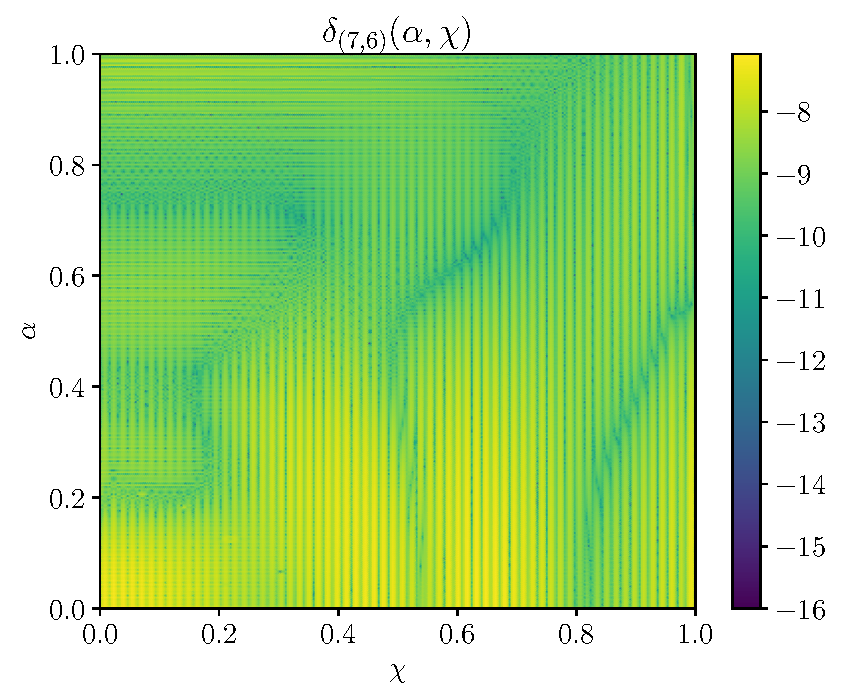
\includegraphics[width=0.95\linewidth]{figures/flux_spline_error.pdf}
    \caption{Different rescalings and reparametrizations of the flux to improve interpolation accuracy of the numerical data.}
    \label{fig:fluxSplineError}
\end{figure}

\begin{figure}[bhtp]
    \centering
    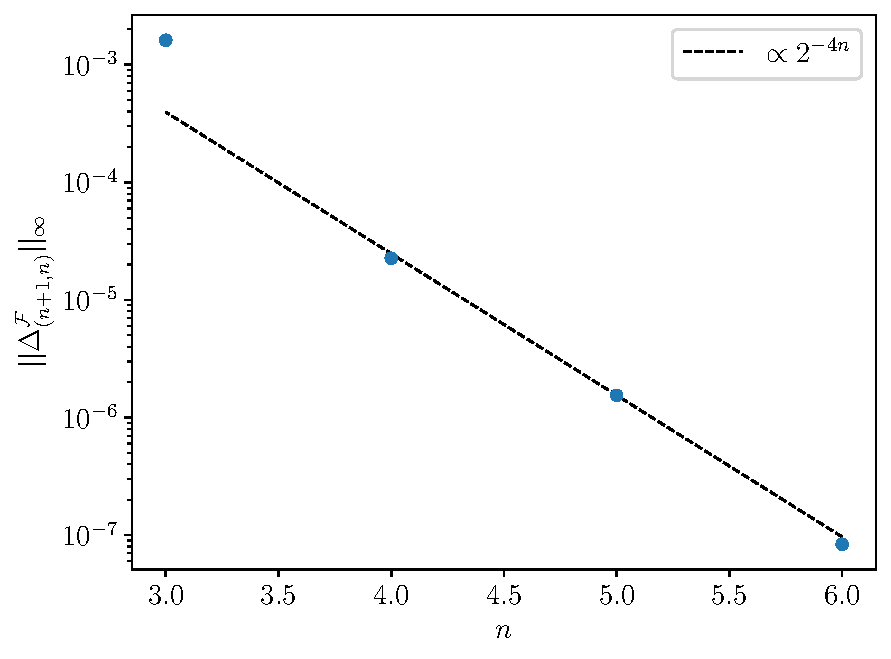
\includegraphics[width=0.95\linewidth]{figures/spline_convergence.pdf}
    \caption{Different rescalings and reparametrizations of the flux to improve interpolation accuracy of the numerical data.}
    \label{fig:fluxSplineConvergence}
\end{figure}

\begin{figure*}[bhtp]
    \centering
    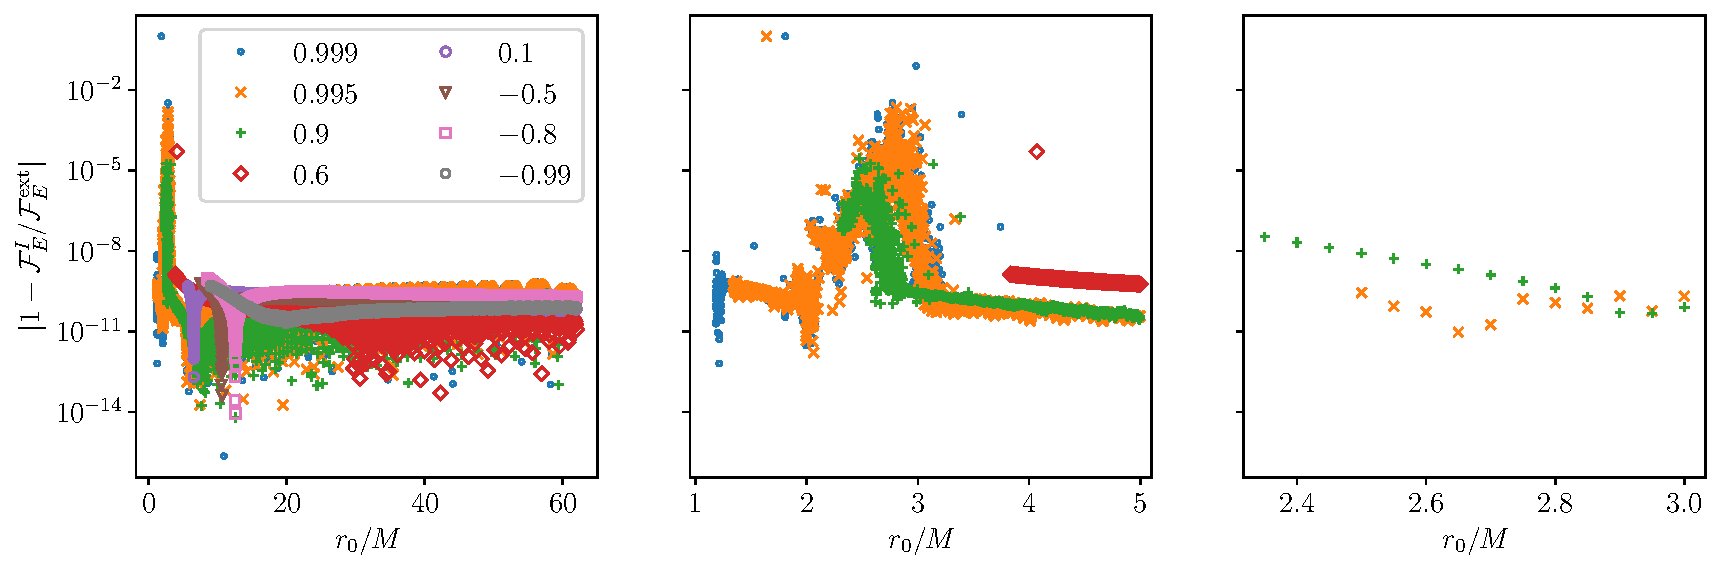
\includegraphics[width=0.95\linewidth]{figures/flux_comparison.pdf}
    \caption{Different rescalings and reparametrizations of the flux to improve interpolation accuracy of the numerical data.}
    \label{fig:fluxComparison}
\end{figure*}

\begin{figure}[bhtp]
    \centering
    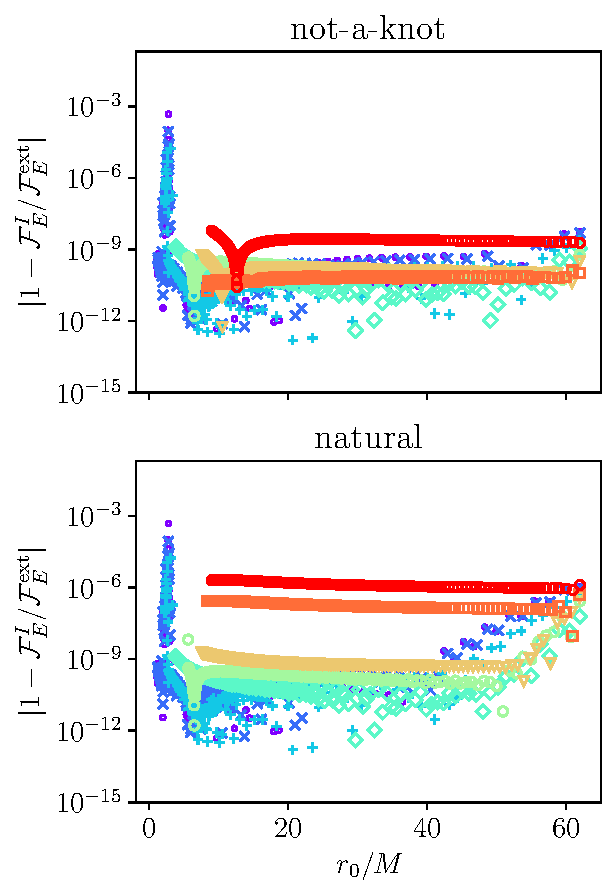
\includegraphics[width=0.95\linewidth]{figures/boundary_condition_comparison.pdf}
    \caption{Different rescalings and reparametrizations of the flux to improve interpolation accuracy of the numerical data.}
    \label{fig:fluxComparison2}
\end{figure}



To confirm the numerical accuracy of our interpolated data, we perform a series of comparisons and self-consistency checks. First we assess the accuracy of our flux interpolant by downsampling the data. Let $f^I_{(n,m)}(x,y)$ denote a bicubic spline that interpolates the function $f(x,y)$ using $(2^n+1) \times (2^m+1)$ grid points in $(x,y)$, e.g., $\mathcal{F}_{N(8,7)}^I(\alpha, \chi) = \mathcal{F}_N^I(\alpha, \chi) $. We then estimate the fractional interpolation error for the flux spline $\mathcal{F}_{N(N',M')}^I$ via
\begin{align}
    \delta_{(N',M')}(\alpha, \chi) = \left|1 - \frac{\mathcal{F}_{N(N',M')}^I(\alpha, \chi)}{\mathcal{F}_{N(N'+1,M'+1)}^I(\alpha, \chi)} \right|.
\end{align}
By downsampling the data, we calculate $\delta_{(7,6)}$, $\delta_{(6,5)}$, and $\delta_{(5,4)}$. We plot $\delta_{(7,6)}$ in Figure \ref{fig:fluxSplineError}, demonstrating that $\delta_{(7,6)}<10^{-6}$ across the entire domain. To estimate the interpolation error of our fully-sampled spline, $\delta_{(8,7)}$, we examine the convergence rate of $|| \delta_{(n+1,n)} ||_\infty$ in Figure \ref{fig:fluxSplineConvergence}. We find that $|| \delta_{(n+1,n)} ||_\infty \propto 2^{-4n}$, which is consistent with the standard fourth-order scaling for cubic spline errors ($\delta \sim \Delta x^4$ for grid spacing $\Delta x$). Provided this scaling holds true as we increase the sampling rate, we estimate that $\delta_{(8,7)} \lesssim 5\times 10^{-8}$.

We also compare the flux interpolant to Kerr circular flux values produced by independent codes \cite{TaraETC14, GralHughWarb16}. Tables of these values are provided within the ``Circular Orbit Self-force Data'' repository hosted by the Black Hole Perturbation Toolkit \cite{BHPTK18}. Figure \ref{fig:fluxComparison} plots the fractional errors between the Toolkit data set and our interpolated fluxes for the spin values $\hat{a} = [-0.99, -0.8, -0.5, 0.1, 0.6, 0.9, 0.995, 0.999]$ as a function of the orbital separation $r_0$. For $r_0 \gtrsim 3.5 M$ the fractional errors in the fluxes are consistent with the interpolation error estimated in Figure \ref{fig:fluxSplineError}, indicating that our flux results are reliable to a precision $\sim 10^{-9}$ in this domain. Crucially, we find that our use of the $E(3)$ boundary condition in our spline interpolation is essential for achieving these small fractional errors. For example, in Figure \ref{fig:fluxComparison2} we plot the fractional errors resulting from the use of the more common `natural' or `not-a-knot' spline boundary conditions when interpolating our flux results. Both boundary conditions degrade the accuracy of our interpolated flux data, with the natural spline providing the largest fractional errors. For both the natural and not-a-knot splines, the fractional errors rise as we approach larger negative values of the spin ($a \rightarrow -1$) and larger orbital separations ($\Omega \rightarrow \Omega_\mathrm{min}$), where our flux data is sparsely-sampled. Therefore, a careful choice of boundary conditions can significantly improve the accuracy of our splines, thereby diminishing the number of points at which we need to perform expensive calculations of the gravitational wave fluxes.

Finally, we return the near-ISCO region of Figure \ref{fig:fluxComparison}. The fractional errors between our data and the fluxes published in the Toolkit peak at $\sim 10^{-3}$ near $r_0 \sim 3 M$, as seen in the middle plot of Figure \ref{fig:fluxComparison}. To identify the source of this disagreement, we perform another set of flux calculations using the \texttt{Teukolsky} Mathematica package \cite{BHPT_TEUK}, which is also provided in the Black Hole Perturbation Toolkit.\footnote{Note that this package was designed and implemented independently of the circular flux data published in the ``Circular Orbit Self-force Data'' Toolkit data repository.} In the Mathematica code, we use over 300 digits of precision to guarantee the accuracy of the computed flux values. The fractional error between our flux interpolant and the high-precision Teukolsky fluxes are shown in the right plot of Figure \ref{fig:fluxComparison}, demonstrating strong agreement between our data and the Toolkit-generated fluxes. Therefore, we suspect that the flux values published in the ``Circular Orbit Self-force Data'' repository are not accurate to all reported digits for $ 2M \lesssim r_0 \lesssim 4 M$.

Altogether, these tests indicate the the error in our interpolated flux function is $< 10^{8}$ and often matches the intrinsic error in the underlying flux data, which was calculated to a requested precision of $\sim 10$ digits. Since flux errors scale as $\sim \epsilon^{-1}$ over an inspiral, we expect that this level of flux interpolation error will have a subradian impact on the phase accuracy of our gravitational waveforms for astrophysically-realistic systems.

\subsection{Numerical accuracy of trajectories}
\label{app:trajtests}

Next we validate the accuracy of our trajectories. For the time and phase evolution, we are concerned with the absolute error in the splines, since the quantities $\Omega t$ and $\Phi$ appear directly in the phasing of our frequency- and time-domain waveforms, respectively. 

First we verify the numerical convergence of our splines. Similar to our analysis of the fluxes, we define the convergence measures,
\begin{align}
    \Delta^t_{(N',M')} &= \left| {\check{t}^I_{(N',M')}} - {\check{t}^I_{(N'+1,M'+1)}} \right|,
    \\
    \Delta^\Phi_{(N',M')} &= \left| {\check{\Phi}^I_{(N',M')}} - {\check{\Phi}^I_{(N'+1,M'+1)}} \right|,
\end{align}
and plot $|| \Delta^{t/\Phi}_{(n+1,n)}||_\infty$ for $n = (3, 4, 5, 6)$ in Figure \ref{fig:trajConvergence}. As before, the error improves as we increase the sampling density by a factor of $2$ in each dimension, though in this case the maximum absolute error converges slightly faster than $2^{4n}$. Thus extrapolating this rate of convergence, we estimate $|| \Delta^{t/\Phi}_{(8,7)}||_\infty \lesssim 5\times 10^{-7}$. 

Next, we check that the interpolated trajectories satisfy the equations of motion \eqref{eqn:eom2} via the two tests,
\begin{align}
    \delta_{t}(\hat{\Omega}_0, \hat{a}) &= \left| 1 - \left[1 + \frac{1}{\mathcal{F}^I_N}\left(\frac{\partial\mathcal{E}}{\partial\alpha} \right)\right]\left[1 - \frac{d\check{t}^I}{d\alpha}\right]^{-1}\right|,
    \\
    \delta_{\Phi}(\hat{\Omega}_0, \hat{a}) &= \left| 1 -  \left[1 + \frac{\hat{\Omega}_0}{\mathcal{F}^I_N}\left(\frac{\partial\mathcal{E}}{\partial\alpha} \right)\right]\left[1 -\frac{d\check{\Phi}^I}{d{\alpha}} \right]^{-1}\right|,
\end{align}
where, on the righthand side, all functions and derivatives are evaluated at $\alpha(\hat{a},\hat{\Omega}_0)$ and $\chi(\hat{a})$. We shift the numerators and denominators by a factor $1$, because the $\alpha$-derivatives vanish at $\alpha = 0$. This translation effectively leads to $\delta_t$ and $\delta_\Phi$ measuring absolute error for values of $\alpha \lesssim 0.05$, while measuring relative error for values $\alpha \gtrsim 0.05$. Based on this analysis, we find $||\delta_t||_\infty \simeq 10^{-5.8}$ and $||\delta_\Phi||_\infty \simeq 10^{-5.9}$.

To assess the accuracy of $\hat{\Omega}^I(\check{t};\hat{a})$, we calculate the error
\begin{align}
    \delta_{\Omega}(t_0, \hat{a}) = \left| 1- \frac{t_0}{\check{t}^I[\alpha(\hat{\Omega}^I[\beta(t_0)])]} \right|,
\end{align}
where once again all functions are evaluated at $\chi(\hat{a})$.

\bibliography{parent}

\end{document}
